

\documentclass[
thesis  % please do not delete or change this line!
]{csthes}

%\documentclass[12pt]{report}

% The following packages are loaded automatically. Do not load them
% manually as you might risk an option clash:
%   -babel (heading translation and hyphenation)
%   -natbib (citing, see www.ctan.org/tex-archive/macros/latex/contrib/natbib/natbib.pdf)
%   -fancyhdr (headers and footers)
%   -fontenc (output encoding)

% Set the encoding your tex-source is written in.
% Use utf8 if possible. Other options that might 
% work for you are:
%   latin1 (Unix/Linux or Windows)
%   ansinew (Windows)
%   applemac (Mac)
\usepackage[utf8]{inputenc}

%for tables
\usepackage[table,xcdraw]{xcolor}
\usepackage{makecell}
\usepackage{array}
\newcolumntype{L}{>{\centering\arraybackslash}m{3cm}}
\renewcommand\theadfont{\bfseries}


%for graphics
\usepackage{graphicx}
\usepackage{subcaption}

% for pseudo algorithms
\usepackage{algpseudocode}
\usepackage{algorithm2e}

% For the online version enable hyperlinks
\usepackage{hyperref}

\usepackage{amsmath}

\usepackage{multirow}


\setlength{\tabcolsep}{6pt}
\renewcommand{\arraystretch}{1.5}

\usepackage{rotating}

\usepackage{tabularx}
\usepackage{booktabs}

\usepackage{float}

\usepackage[numbers]{natbib}

\usepackage[margin=3.2cm]{geometry}

\usepackage[skip=10pt plus1pt, indent=30pt]{parskip}
%%%%%%%%%%%%%%%%%%%%%%%%%%%%%%%%%%%%%%%%%%%%%
%  Set information about your thesis here  %
%%%%%%%%%%%%%%%%%%%%%%%%%%%%%%%%%%%%%%%%%%%%%
\title{Digital Video Stabilization \\ of an Oscillating Camera \\
using an \\ Inertial Measurement Unit}
\subtitle{}% optional
\setthesistype{Master}
\author{Ibad Rather \matr{1532894}}

\degree{MS Mechatronics}
\supervisor{\\ University: Prof. Dr. Ing. Bhaskar Choubey \\Company: Dr. Steffen Urban 
            }% most likely

% Start of content
\begin{document}
% First set the title page
\maketitle
% Give a short summary of your thesis
\begin{abstract}
Video stabilization is ubiquitous in today's smartphones and action cameras. However, instead of classical “post-processing” image stabilization where image features are extracted and tracked over time [1] or modern deep learning based methods using dense optical flow [2], they need to perform the motion estimation on constrained hardware systems and with very high  frame-rates of up to 100 fps or more. 

Hence the motion estimation, that is necessary to correct vibrations, shaking or rolling shutter distortions is performed using Inertial Measurement Units (IMUs). Typically, the motion estimates are reduced to rotational motions [3] (using gyroscopes) as the distance between frames is small and the field-of-view of the lenses large $(\geq 50^\circ)$. In addition, estimating translational motion is a difficult challenge using low-cost IMUs as the double integration of accelerometer readings is prone to strong drift and leads to large errors even over short time periods $(\leq 1s)$. 

This thesis should investigate and develop an image stabilization method for an oscillating camera. The camera has a small field-of-view and hence small translational movements along the viewing direction will be visible and need to be stabilized. The camera is coupled with an IMU and attached to a linear stage, that will mimic the oscillating movements. The camera records a monitor or a static target. An additional goal is the implementation, optimization and testing of the proposed algorithm on a modern embedded chip.

\end{abstract}
% Set the table of contents
\tableofcontents%

% And other tables/lists optionally
\listoftables%
\listoffigures%

% Start the main work (handles page numbering etc.)
\mainmatter

% While writing your thesis it is advisable to only load the chapter you are currently working on. It decreases the compile time. 

% 1. Chapter: ''Introduction''
\chapter{Introduction} \label{chapter_one}

An introduction gives the motivation of your work:
\begin{itemize}
\item What is the topic?
\item Why is this relevant?
\item Why is this exciting?
\item What concrete problem do you want to solve?
\end{itemize} 
State clearly your research question. \\
The end of the introduction gives an advanced organizer for the rest of the thesis, i.e., a sentence for each chapter.

Typically you cite in one of the following ways: This algorithm is based on {\sc GraphPlan} \citep{Blum97}. \citet{Blum97} introduced {\sc GraphPlan} as an efficient algorithm for plan construction for finite domains.


% Start: Digital Video Stabilisation
\section{Image Stabilisation}
Stabilising images against camera movements.

\subsection{Hardware Image Stabilisation}
Compensate camera movements with hardware. Expensive.

\subsection{Digital Image Stabilisation}
Compensate movements in post-processing. Economical.
% End: All Information About IMU

% Start: All Information About IMU
\section{Inertial Measurement Unit}
IMU Sensor

\subsection{Noise Models}
About Noise in IMU Sensors

\subsection{Challenges in Working with IMU}
Various Challenges
% End: All Information About IMU
% 2. Chapter: ''Fundamentals Blocks''
\chapter{Fundamental Blocks} \label{chapter_two}

In the previous chapter I discussed the importance of Video Stabilization and the challenges associated performing it using an IMU sensor. This chapter discusses current techniques available to us and also we make a case for our chosen technique. Then we will also discuss in depth the challenges associated with IMU pose-estimation and how we can overcome those challenges. Fundamentals of neural networks and their applications will also be briefly conferred as they are a huge part of this work.

\section{Video Stabilization}
\label{sec:image_stab}
If a camera is not stationary during video capture the output video quality may degrade and not look good. Depending on the movements during capture, the video may look very shaky or even the subjects may not be properly visible. This is very undesirable and can cause visual discomfort \citep{jia2012probabilistic}. One solution to this is to keep the camera steady by mounting it on stable tripod or to a rigid object. But this is not practically possible all the time. There are various scenarios in which the camera may move around a lot and the movements may not be smooth at all e.g an action camera mounted on a helmet or a bicycle, a camera mounted on a car or a robot in wild or some move-able rig or a robot arm.

The motion of the camera can be high-frequency tremors due to vibration, shaking or jiggling of the mounting point \citep{ryu2012robust} or low frequency such as movement of handheld camera during walking \citep{dis_review}. Practically, in most of the video recording scenarios, the camera will have some movement. The goal of video stabilization is to create a output video with same visual content without the undesired movements. 

% Start: Video Stabilization
\subsection{Types of Video Stabilization}
To deal with such movements and to make the video stable various techniques exist. These techniques can be grouped in two categories:

\begin{itemize}
\item Hardware Video Stabilization
\item Digital Video Stabilization  
\end{itemize}
There are techniques which combine both these methods and are called hybrid video stabilization techniques.

The goal of each of these stabilization techniques is to estimate the motion or pose and then use the estimated motion to stabilize the video. Motion/pose estimation will be discussed in the section \ref{sec:pose_estimation} in detail.


\subsubsection{Hardware Video Stabilization (HIS)}
Hardware video stabilization at its core means moving the lens or the image sensor or the camera setup itself to counteract these movements while recording the video. The movements of camera can be minimised by the use of mechanical stabilizers like tripods or dollies \citep{5995525}. The use of electronic gimbals for video recording has also increased recently for both professionals and hobbyists. Video can also be stabilized by varying the optical path between lens and the image sensor. This is generally achieved by using electronic motors and IMU sensors to move around the lens or the image sensor or both to cancel out the motions. After the motion has been counter-acted upon, images are captured which results in a stabilized video output as seen in figure \ref{fig:his}. These methods although mostly effective are not perfect and have both advantages and disadvantages.


\begin{figure}[H]
\centering
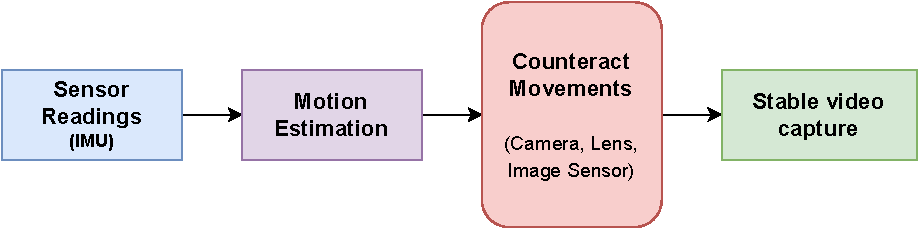
\includegraphics[scale=0.6]{images/fig_chapter2/2_1_his.pdf}
\caption{Hardware Video Stabilization}
\label{fig:his}
\end{figure}

\textbf{Advantages of HVS: }

\begin{itemize}
\item No post-processing for stabilization needed.
\item Works irrespective of the nature of object being captured.
\item Full image without cropping can be used.
\item Shutter Speed of the camera can be reduced
\end{itemize}

\textbf{Disadvantages of HVS:}
\begin{itemize}
\item Camera setups are very bulky.
\item These solutions can be very expensive.
\item More moving parts means higher maintenance.
\item Cannot be improved once hardware is implemented.
\item Not possible on all camera setups.
\end{itemize}

\subsubsection{Digital Video Stabilization (DVS)}
Digital Video Stabilization (DVS) is a software based video stabilization technique \citep{dis_review}. The technique here is similar what is done is HVS i.e. first the motion of the camera is estimated (pose-estimation) and based on this, the image is stabilized. The difference here is that after pose estimation is done, instead of moving around the hardware a suitable transformation (warping) is applied to the image \citep{dis_feat_track} as shown is figure \ref{fig:dis}. The resulting stabilized image (video) is motionless irrespective of the camera motions. DVS is be a very powerful technique but like other methods and techniques, it has its advantages and disadvantages.

\begin{figure}[H]
\centering
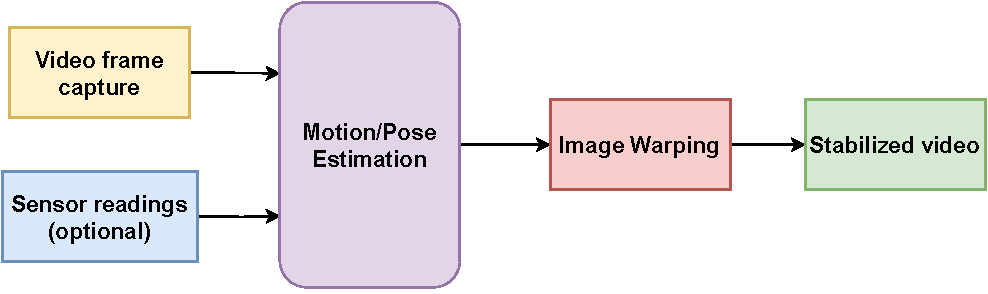
\includegraphics[scale=0.6]{images/fig_chapter2/2_1_dis.pdf}
\caption{Digital Video Stabilization}
\label{fig:dis}
\end{figure}

\textbf{Advantages of DVS: }
\begin{itemize}
\item Cost effective.
\item Smaller camera setups can be used.
\item No changes need to be made to the camera setup for DIS.
\item Can be achieved using IMU sensors for pose estimation which are not very expensive.
\item Can be applied to any video; even the historic ones.
\item Different DIS algorithms can be used on a single video in post processing.
\item Relatively easy to modify DIS software.
\end{itemize}

\textbf{Disadvantages of DVS:}
\begin{itemize}
\item The resolution of the output images (video) is reduced (generally by 5 to 10 percent).
\item May require some manual labour (like in Adobe Premiere Pro: manual feature tracking).
\item Some videos are very difficult (even impossible) to stabilize if there is too much vibration or the features are not visible.
\item May require a lot of computational power (optical flow)
\end{itemize}

Regardless of the type of video stabilization technique motion estimation is a fundamental task and will be discussed in the next section.

% Start: Motion Estimation
\section{Motion Estimation for Image Stabilization}
\label{sec:pose_estimation}
Camera motion (pose) estimation is very important and one of the most challenging parts of image stabilization. Before hardware and digital stabilization techniques/algorithms can be implemented, we need to perform pose estimation to figure out the camera motions. Then based on the actual, shaky camera motions, a smoothed trajectory can be calculated that will create a stabilized video. The accuracy of motion estimation ultimately determines the effectiveness of image stabilization \citep{ryu2012robust}. To estimate the camera motion many sensor and software based techniques exist as show in figure \ref{fig:cam_pose_est}.

\begin{figure}[H]
\centering
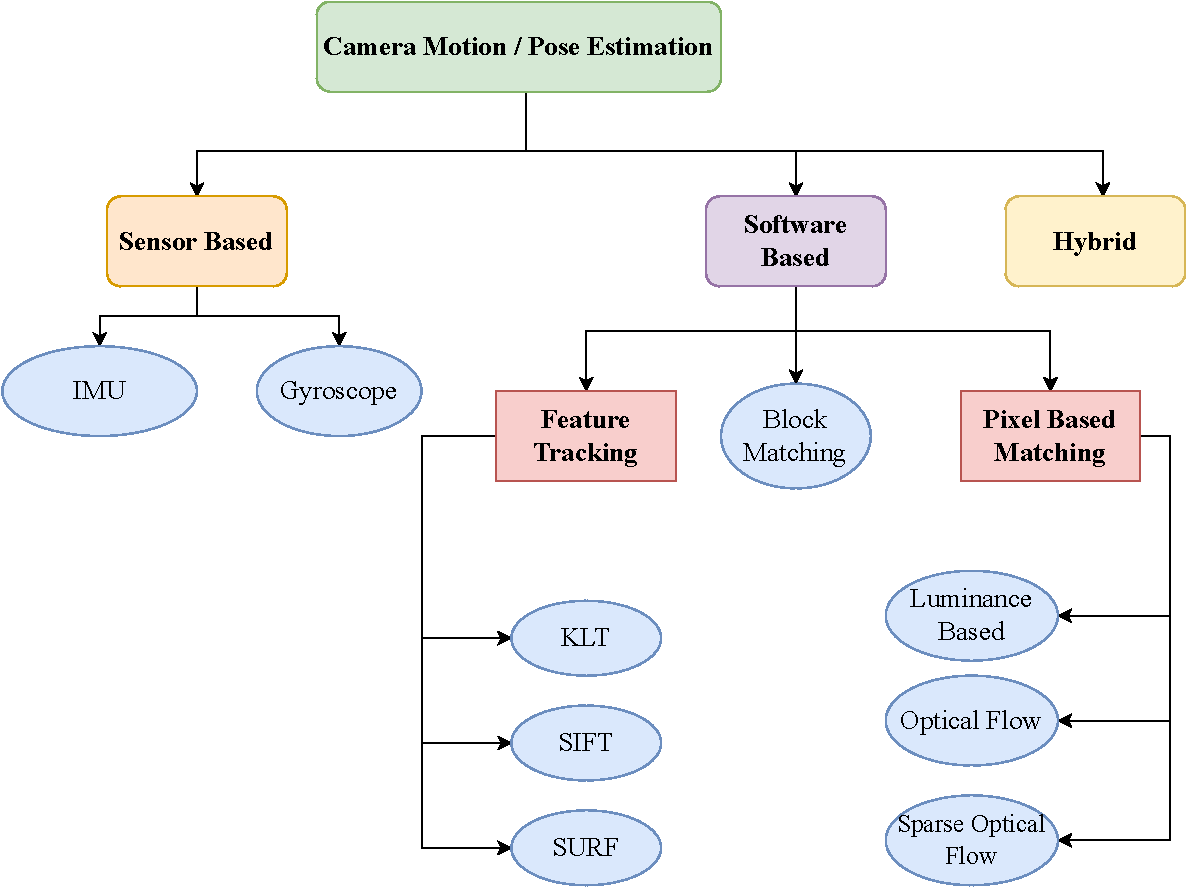
\includegraphics[scale=0.6]{images/fig_chapter2/cam_pose_estimation.pdf}
\caption{Camera Motion/Pose Estimation Techniques}
\label{fig:cam_pose_est}
\end{figure}


\subsection{Software based motion estimation techniques}
\label{sec:software_motion_estimation}
Software based motion estimation techniques/algorithms use the images (frames) coming from the camera for motion estimation and subsequently for stabilization. Some of these software based techniques are listed below \citep{dis_review}:

\begin{itemize}
\item Pixel-based matching
\item Block-Matching
\item Feature-Matching
\end{itemize}

Each of these approaches/algorithms used in motion estimation are briefly discussed in the subsequent sections. This will also lay a foundation for why we are not using any of these techniques for this work.

\subsubsection{Pixel-Based Matching}
This method estimates pose by determining the motion of pixels between two frames \citep{dis_review}. For correspondence determination, luminance of two consecutive frames is assumed to be constant throughout. This poses a problem and there can be many pixels having same luminance, so, other constraints are also needed to obtain a unique solution \citep{dis_review}. 

Finding  \textbf{\textit{Optical Flow}} between two consecutive frame is another method for motion estimation. Optical flow is the distribution of apparent velocities of movement of brightness patterns in an image \citep{horn1981determining}. This gives us important information about the spatial arrangement of the objects viewed and the rate of change of this arrangement \citep{gibson1977analysis}. Using this information, relative motions can be estimated between consecutive image frames. These relative motions can be used for camera motion estimation. Many modern neural network based optical flow algorithms have also been developed recently and are used in image stabilization tasks \citep{deep_opti_stab}. This method achieves very good results but has very high computational requirements.

\subsubsection{Block-Matching}
Block matching techniques use blocks of pixels for motion estimation instead of finding correspondence between pixels of consecutive frames. This allows to remove some ambiguities that occur in pixel-based matching methods \citep{dis_review}. Block-matching approach offers a flexible trade-off between complexity, computational efficiency and accuracy \citep{dis_review} but relies heavily on unambiguous features in the image.

\subsubsection{Feature-Matching (Tracking)}
In these methods, the algorithm first selects the features that are easily recognisable and distinguishable. The motion is estimated by tracking only these features making them computationally less expensive than dense optical flow methods. There are several feature tracking algorithms that are widely used in many computer vision applications.

\paragraph{}\textbf{Kanade Lucas Tomasi (KLT) feature tracker} \citep{tomasi1991detection} is a widely used feature tracking algorithm in computer vision. Features are selected and their position is initialized using this technique and then optical flow is used to track their position \citep{dis_review}.

\paragraph{}\textbf{Scale-invariant feature transform (SIFT)} is also used for motion estimation in digital image stabilization algorithms.  It has been designed for extracting highly distinctive invariant features from images, which can be used to perform reliable matching of the same object or scene between different images \citep{battiato2007sift}. It contains the orientation of the feature in order to be rotation-invariant \citep{dis_review}.

\paragraph{}\textbf{Speeded up robust features (SURF)} is inspired by SIFT but is faster \citep{dis_surf}. This technique is also widely used in feature selection and tracking for motion estimation.

A common theme here in software based motion estimation techniques is to detect features (be it a pixel, or a group of pixels or any other particular image feature) and then tracking it for motion estimation. But, there are certain use cases like ours where feature tracking from frame to frame is very difficult or unreliable. The features in an image sequence can be moving in different directions, which makes reliable motion estimation using these techniques impossible. This might happen it the observed scene is not static and contains many moving objects. This is the case for this work and the goal is to estimate the motion of the camera independent of image observations. To this end inertial sensor based pose-estimation will be used.

\subsection{Sensor based Motion Estimation}
Pose estimation is a huge area of research especially for the field of robotics and autonomous driving. Various sensors can be used for motion estimation, including accelerometers, gyroscopes, magnetometers or satellite navigation systems. To help camera pose estimation generally a combination of gyroscope and accelerometer is used. In combination, these two sensors are called Inertial Measure Unit (IMU). With these two sensors the 6 degree of freedom (DoF) motion of a camera in space is fully observable. For this work, we will be using IMU for pose estimation as using it has many advantages and will make our image stabilization algorithm invariant to moving objects.

% Start: IMU Sensors
\section{Inertial Measurement Unit (IMU)}
\label{sec:imu}
IMU is one of the most commonly used sensors in the world and present all around us in mobile devices, smartwatches, virtual reality gear and cameras. IMU sensors are used in a wide variety of applications like navigation, robotics, drones, smart watches, sports learning, augmented reality systems, industrial quality control \citep{ahmad2013reviews}  and also for image stabilization in cameras. In all these applications, IMU are used for pose estimation in some form; either for absolute pose estimation or change in pose.

An IMU measures acceleration(m/s²) and angular velocity (rad/s). They can make these measurements in multiple degrees of freedom e.g., a 6-DoF IMU sensor includes a 3-axis accelerometer (x, y, z) and 3 axis gyroscope (x, y, z) \citep{constant2021data}. The accelerometer will make independent acceleration measurements in these axis. Similarly, the gyroscope makes independent angular velocity measurements about these three axis.



There are a lot of reasons to use IMUs and these reasons are surely a very huge contributor to them being one of the most commonly used sensors in the world. There are different types of IMUs e.g., optical, laser and Micro-electro-mechanical systems (MEMS) IMUs. All these different types of IMUs record similar measurements but have different characteristics, sizes, accuracy and prices. MEMS IMUs are the scope of this work as they have various qualities that make them the best fit for DVS. Some of their qualities are \citep{woodman2007introduction}.:

\begin{itemize}
\item They have small size
\item low weight
\item rugged construction 
\item low power consumption 
\item cheap
\item high reliability 
\item low maintenance
\item can be used in hostile environments 
\end{itemize}

\subsection{Pose Estimation with IMUs}
In this thesis, a pose has six degrees of freedom and is defined by a position and a orientation with respect to some coordinate system. Continuous IMU readings are taken and using some algorithm pose is estimated. Figure \ref{fig:strapdown_imu} below shows the strap-down inertial navigation algorithm \citep{woodman2007introduction}. For orientation estimation gyroscope readings are used and for position estimation both gyroscope and accelerometer readings are used. The use of this algorithm directly for pose-estimation is not possible as the IMU readings are far from being ideal, they contain noise and have a bias \citep{woodman2007introduction} which needs to be accounted for. In addition, integration of the accelerometer signal needs prior information like the initial velocity or the initial position that are, dependent on the application, not always easily obtainable.

\begin{figure}[H]
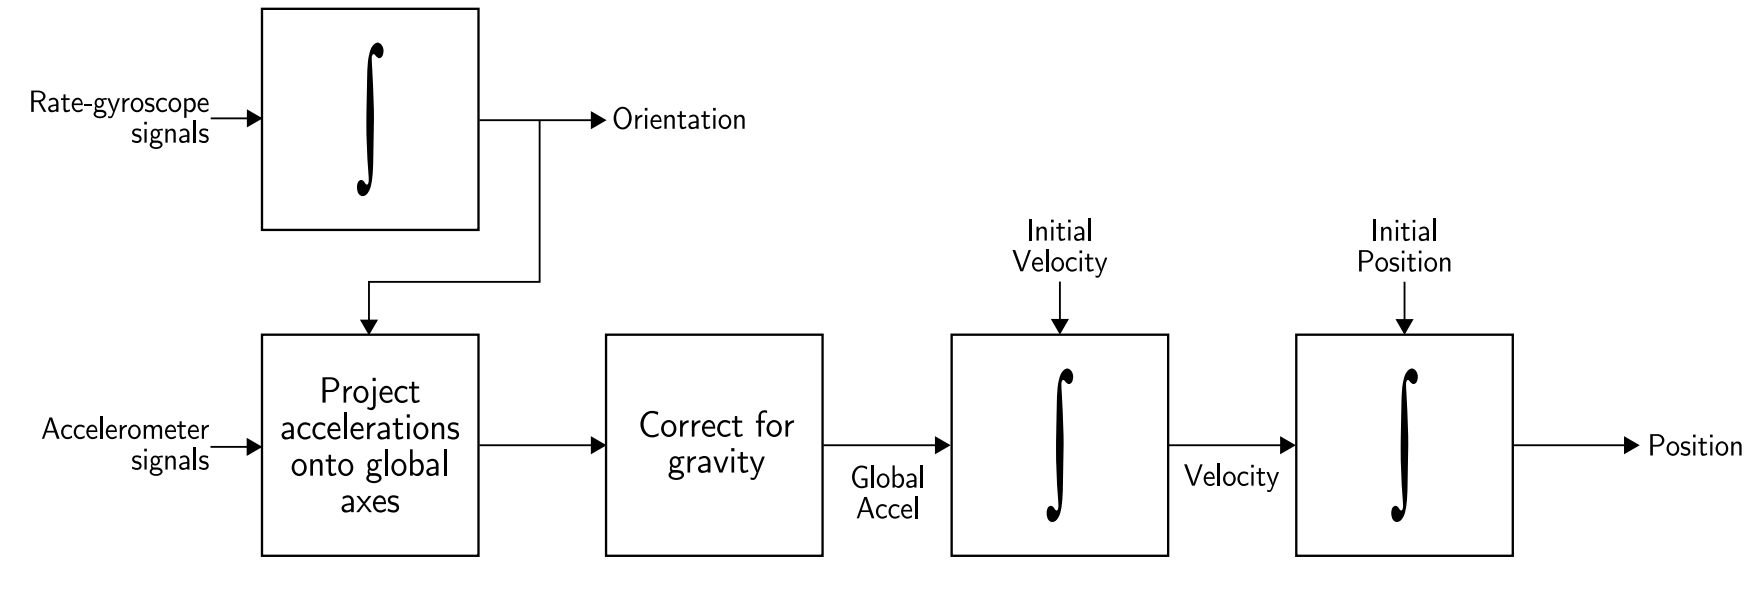
\includegraphics[scale=0.2]{images/fig_chapter2/strap_imu_algo.png}
\caption{Strap-down inertial navigation algorithm \citep{woodman2007introduction}}
\label{fig:strapdown_imu}
\end{figure}

\subsection{IMU Noise Models}
MEMS sensor outputs are inherent to noise and there is different types of noise with which we have to deal. For IMUs, the readings coming from a sensor could be modelled as a combination of three entities: true signal, bias and white noise.

\textbf{Gyroscope}
\begin{equation}
    \omega_{n}(t) = \omega(t) + b_{g}(t) + n_{g}
\label{eqn:gyro_noise}
\end{equation}

Where $ \omega_{n}(t) $ is the noisy gyroscope signal, $ \omega(t) $ is the true gyroscope signal, $ b_{g}(t) $ is the gyroscope bias and $ n_{g} $ is the gyroscope white noise.

\textbf{Accelerometer}
\begin{equation}
    a_{n}(t) = a(t) + b_{a}(t) + n_{a}
\label{eqn:accel_noise}
\end{equation}

Where $ a_{n}(t) $ is the noisy accelerometer signal, $ a(t) $ is the true accelerometer signal, $ b_{a}(t) $ is the accelerometer bias that is time varying and $ n_{a} $ is the accelerometer white noise.

To visualise the \textit{Noise Model}, let's take a true unit signal as show in figure \ref{fig:imu_noise}. \textbf{Bias} can be defined as constant offset from true signal value. White noise can be thought of as random fluctuations of equal intensity and different frequency from the true value of the signal (\ref{fig:imu_noise}).

\begin{figure}[H]
  \begin{subfigure}{\linewidth}
  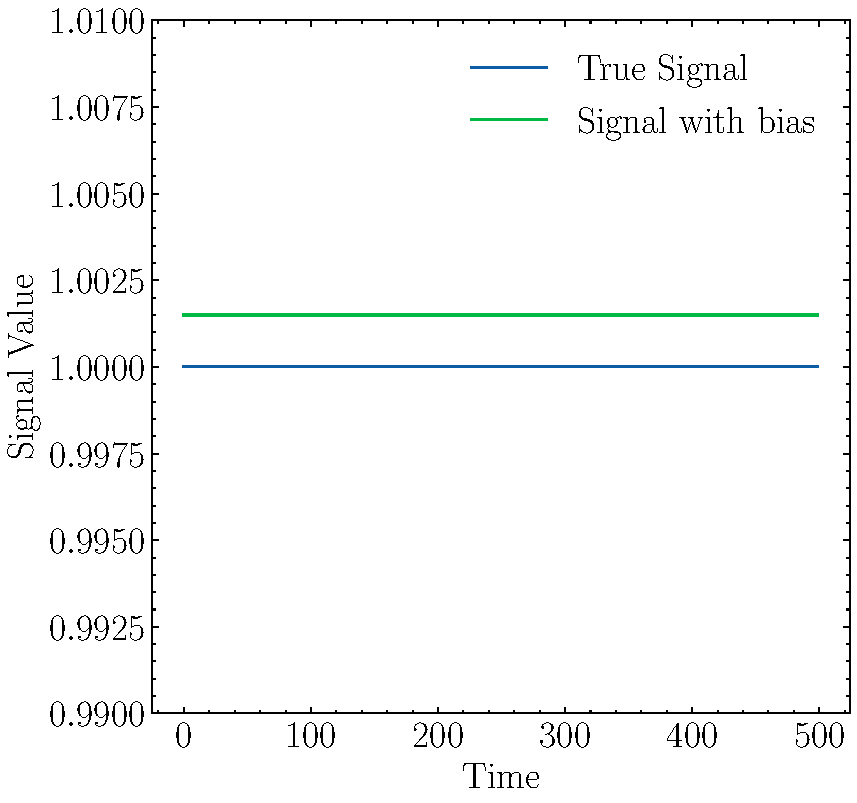
\includegraphics[width=.5\linewidth]{images/fig_chapter2/noise_figs/signal_with_bias.pdf}\hfill
  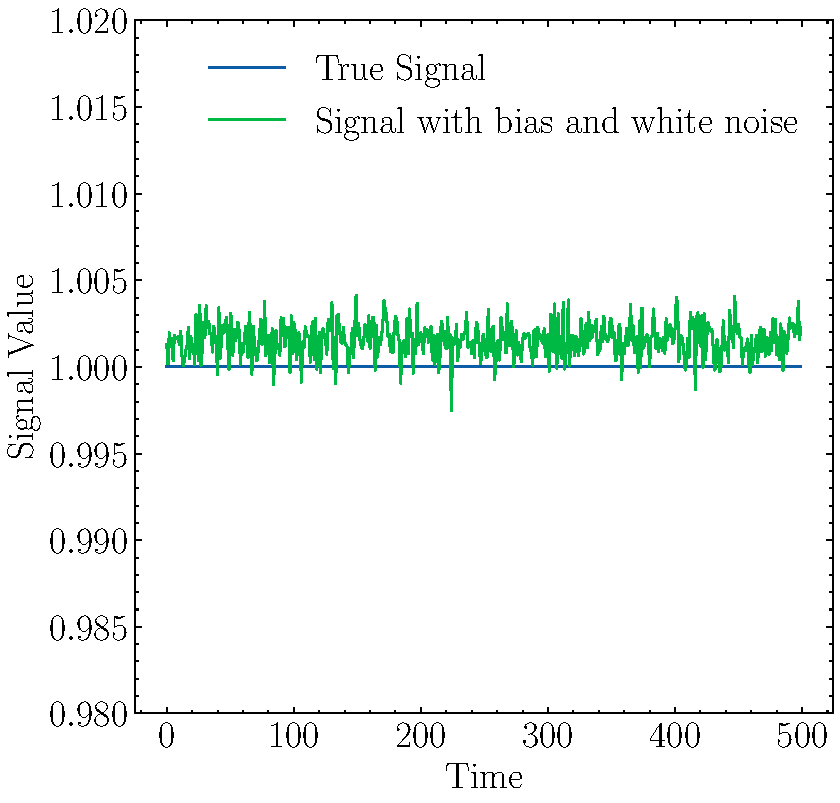
\includegraphics[width=.5\linewidth]{images/fig_chapter2/noise_figs/signal_with_bias_and_noise.pdf}
  \end{subfigure}\par\medskip
  \caption{IMU noise model visualisation}
\label{fig:imu_noise}
\end{figure}

For both gyroscope and accelerometer the signal can be independently modeled this way in each of its axis (x, y and z) \citep{imu_noise}. As you can see from the plots, the noisy signal looks very different from the true signal. Using the noisy signal directly for pose estimation can lead to very inaccurate results. Although the modelling equation looks the same for both gyroscope and accelerometer, but they have different effects on pose estimation as the strap-down inertial algorithm suggests. So, there are different challenges associated with position and orientation estimation using this sensor with absolute position estimation being especially difficult.

\subsubsection{Gyroscope Error Characteristics}
To get orientation from the gyroscope, the readings need to be integrated once and the global orientation needs to be updated. Doing this continuously with the noisy signal will result ill result in erroneous orientation tracking and ultimately in a drift of the absolute rotation even if the device is stationary. Hence methods are needed to estimate the sensor errors, especially the bias. In table \ref{tab:imu_error_char} you can see all the errors and effect of those on orientation measurement.

\subsubsection{Accelerometer Error Characteristics}
Generating position information from accelerometer is not a single step like in case of Gyroscope. Based the strap-down inertial navigation algorithm shown in figure \ref{fig:strapdown_imu} there are multiple steps involved. First, the accelerometer readings need to be projected onto the global navigation frame using the orientation calculated from gyroscope. Then, the accelerometer reading needs to be corrected for gravity. After that we double integrate the signal based on initial velocity and initial position to finally get the position.

So, there is double integration present in the algorithm. We also have a noisy signal, so, the noise also gets integrated two times. This can result into very inaccurate position estimations and is one of the most challenging parts of working with an IMU. In table \ref{tab:imu_error_char} you can see all errors in an MEMS accelerometer and effect of those on position measurement.

% imu error table
\begin{table}[H]
\centering
\begin{tabular}{ l| L| L }
     Error Type & Description & Result of Single/Double Integration \\ 
     \hline
     Gyroscope bias & 
     A constant bias $ \epsilon $ & 
     Steadily growing angular error.  \[\theta(t) = \epsilon(t)\] \\
     \hline
     Gyroscope white noise & 
     White noise with some standard deviation $ \sigma $ & 
     An angular random walk, whose standard deviation grows with the square root of time. 
     \[\sigma_\theta(t) = \sigma \sqrt{\delta t}\] \\
     
     \hline
     Accelerometer bias & 
     A constant bias $ \epsilon $ in the accelerometer's output signal. & 
     A quadratically growing position error. \[s(t) = \epsilon  \frac{t^{2}}{2}\]   \\
     \hline
     Accelerometer white noise & 
     White noise with some standard deviation $ \sigma $ & 
     A second order random walk. The standard deviation of the position error grows as
     \[\sigma_s(t) = \sigma  t^{\frac{3}{2}}  \sqrt{\frac{\sigma  t}{3}}\]   \\
     
\end{tabular}
    \caption{Summary of IMU error sources \citep{woodman2007introduction}}
    \label{tab:imu_error_char}
\end{table}

\subsubsection{Challenges in Working with IMUs}
For the reasons mentioned in the previous sections, it is not straightforward to work with IMUs, especially for absolute position estimation as the errors introduced are squared with time. This results in a \textbf{drift} from actual position, which for any image stabilization algorithm is very detrimental. Orientation estimation is still relatively reliable over short periods of time and is the main reason why gyroscope based hardware as well as digital video stabilization is more common.

% Start: Pose Estimation
\section{Pose Estimation using IMU}
Based on the strap-down inertial navigation algorithm (Section \ref{fig:strapdown_imu}) and Newtonian mechanics, pose can be estimated from the IMU readings using equation \ref{eqn:ori_imu_readings} and equation \ref{eqn:pos_imu_readings}. We need a history of pose for the iterative pose estimation to work. $ \omega $ and $ a $ are the gyroscope and accelerometer readings respectively as defined in section \ref{sec:imu}.

\begin{equation}
  \label{eqn:ori_imu_readings}
  \begin{aligned}
    O(t) = O(t - dt) exp(\int_{t-dt}^{t} \Omega(t) dt) \\
  \end{aligned}
\end{equation}

 Orientation $ O(t) $ is the updated orientation in global frame at current timestamp using orientation at previous timestamp $ O(t - dt) $  and the sensor readings $ \Omega(t) $ as shown in equation \ref{eqn:ori_imu_readings}.

\begin{equation}
  \label{eqn:pos_imu_readings}
  \begin{gathered}
    a_g(t) = O(t)a(t) \\
    v(t) = v(t-dt) + (a_g(t) - g_g)dt \\
    P(t) = P(t-dt) + v(t)dt
  \end{gathered}
\end{equation}

 Position estimation can be done using a series of mathematical equations as shown in equation \ref{eqn:pos_imu_readings}. The accelerometer readings are first projected onto the global axis based on the orientation $ O(t) $. Then the current velocity $ v(t) $ is calculated by integrating the acceleration $ a_g(t) $ and adding it to velocity at previous time-step $ v(t-dt) $. Finally, to get the current position $ P(t) $ we integrate the velocity $ v(t) $ add it to the previous position. 

These equations are the backbone for classical pose estimation algorithms using IMU sensors. Bias and white noise present in the sensor readings also integrates causing a \textbf{drift} in estimation. In case of Gyroscopes, white noise causes an \textit{angular random walk} whose standard deviation grows proportionally with square root of time \citep{woodman2007introduction}. And leaving the bias unaccounted for causes an orientation error growing linearly with time as shown in table  \ref{tab:imu_error_char}. In case of accelerometer the drift is aggravated because the orientation error is also contributing to it. The subtraction of gravity $ g $ from the readings is not perfect either and causes further drift. The bias in the readings also increases the error (hence the drift) quadratically with time. On top of all these errors the effect of white noise  is a \textit{second order random walk} whose standard deviation increases quadratically with time as shown in table \ref{tab:imu_error_char}.

We can very comfortably conclude that using the inertial navigation system in its pure form is not possible for accurate pose estimation with MEMS IMUs. There are several techniques which can be used to diminish the effect of the noise and the bias. Bias can be estimated for any IMU by keeping it stationary for a few seconds  (for the accelerometer this is only true if any axis is perfectly aligned with the gravity axis). The readings that we get for a stationary IMU sensor is the bias for that sensor. Then this bias can be adjusted in the signal recorded during operation.

But modern learning based methods do not use these equations. Instead they are more data driven and let the neural network infer these relations based on the training data.

\subsection{Classical Techniques}
IMUs have been used extensively for pose estimation for the better half of the century and were used to track the Apollo 11 rocket that took man to the mars. Over the years many techniques and algorithms have been developed to improve pose-estimation accuracy using IMUs. These techniques range from simple signal filtering to more advanced state-estimation algorithms.

\subsubsection{Signal Filtering}
There are also various signal-processing techniques that can be used to reduce the white noise. Noise can be characterised as a high-frequency content in any signal. Therefore, we can use simple filters like a low pass filter or a moving average filter with big horizon to eliminate the noise up to some extent. These techniques are in no way perfect and may even cause loss of true signal if not configured properly.

\subsubsection{Kalman Filter}
Kalman filters are very useful for estimation purposes. They can be used to estimate pose using an IMU sensor by filtering noise based on a covariance matrix \citep{ferdinando2012embedded}. The values of this covariance matrix can be varied but there is a trade-off between noise sensitivity and accuracy. Kalman filter is used to fuse multiple sensors to improve the accuracy of estimation. But in our case the accuracy it provides over time is not enough (\citep{kok2017using}, \citep{alatise2017pose}, \citep{bangera2020mems}) which has been evaluated already internally and hence cannot be used.

These techniques may be good enough for some other applications, but in our case their use is not enough. The precision requirements are very high. Even with the use of these algorithms, there is still a drift present which is unacceptable for this use case.

\subsection{Neural Network Based}
With the advancement of neural networks and their ability to outperform classical algorithms in many domains, over the years many techniques have been developed to solve the challenge of double integrating accelerometer readings. Based on the fact that the vibrations in our camera setup have similar motion characteristics and patterns, a neural network can learn these pattern and make accurate predictions. Some of the techniques which laid the foundation of the methodology we used are discussed in chapter \ref{chapter_three} of this report.


\section{Neural Network Architectures}
The evolution of neural networks and deep learning techniques over the past decade has made the use data driven approaches very common. Data driven approaches have surpassed classical techniques in many applications. There are various neural network architectures, their variations and combinations present today. Each of these architectures have properties that aid in achieving solutions for various challenges.

\subsection{Multi Layer Perceptron (MLP)}
MLPs are the simplest form of Artificial Neural Networks (ANNs) or Deep Neural Networks (DNNs) and are made of a combination of perceptrons/ neurons (figure \ref{fig:perceptron}). An MLP has at-least three layers; an input-layer, a hidden layer and an output-layer as shown in figure \ref{fig:mlp}. During the training phase the weights of the network are adapted using back-propagation (\citep{rumelhart1986learning}) to minimize a target loss function (gradient descent). These networks act as universal function approximators \citep{cybenko1989approximation} and therefore are used to create mathematical models by regression analysis. We will be using MLPs as Fully Connected (FC) layers in all of our networks for this purpose.

\begin{figure}[H]
    \centering
    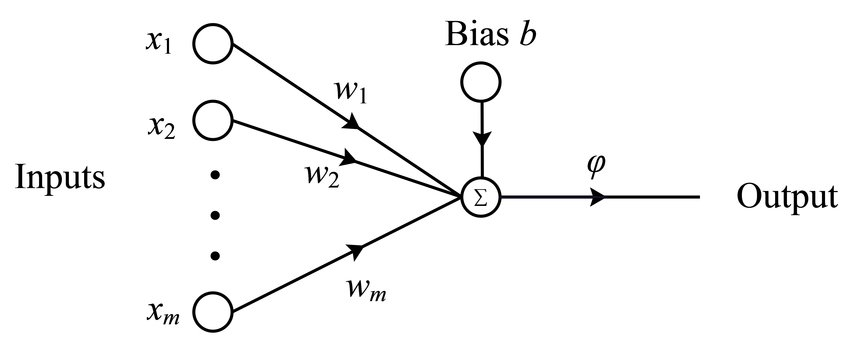
\includegraphics[scale=0.5]{images/fig_chapter2/nns/perceptron.png}
    \caption{Perceptron}
    \label{fig:perceptron}
\end{figure}

\begin{figure}[H]
    \centering
    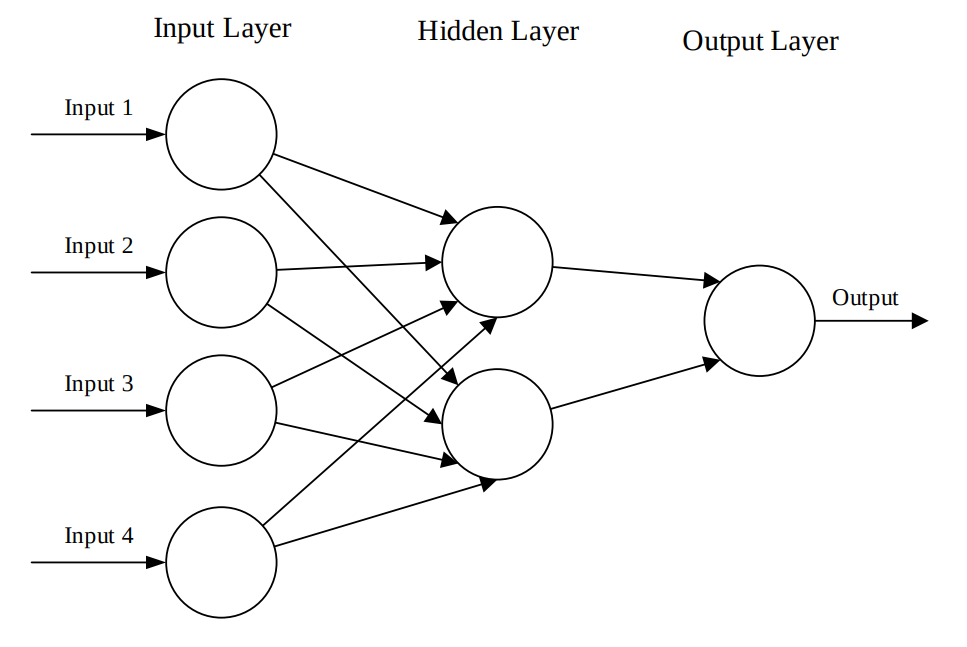
\includegraphics[scale=0.3]{images/fig_chapter2/nns/mlp.png}
    \caption{Multi Layer Perceptron}
    \label{fig:mlp}
\end{figure}

\subsection{Convolutional Neural Networks (CNNs)}
CNNs are another class of ANNs and are responsible for revolutionising the field computer vision and has applications in Natural Language Processing, Recommender Engines and Time Series as well. These networks also have neurons that optimise through learning \citep{cnn2015introduction}. These networks are capable of learning multiple features from the data by abstracting the data into feature maps. In our case we input a 6 channel (3-accelerometer and 3-gyroscope) data and then the CNNs take the data from 6 channels to 64 channels (tensor maps). Then these features are fed into the Fully Connected Layers (FC / MLP) at the end to regress the pose as shown in figure \ref{fig:cnn_fc}. This also results in reducing dimensionality of the data while regressing the output. 

\begin{figure}[H]
    \centering
    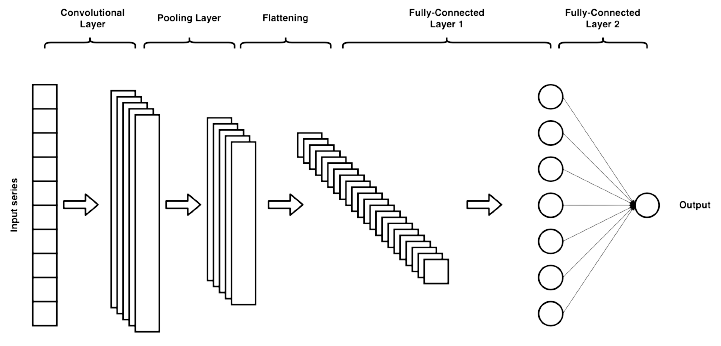
\includegraphics[scale=0.4]{images/fig_chapter2/nns/cnn_mlp.png}
    \caption{CNN layers with FC layers}
    \label{fig:cnn_fc}
\end{figure}

\subsection{Transformers}
Transformer architecture as shown in figure \ref{fig:transformer_arch} is one of the latest proposed neural network architectures that has outperformed its predecessors. Its use mainly started for natural language processing \citep{vaswani2017attention} but was also adopted for computer vision \citep{dosovitskiy2020image}. The use of transformers is also extended for Inertial based Human Activity Recognition (HAR) \cite{shavit2021boosting} and Inertial Navigation \citep{rao2022ctin}. This architecture adopts Multi Headed Attention Mechanism (MHA) \citep{vaswani2017attention} which results in weighing the significance of each part of input data. This significantly improves performance of the network as it learns the importance of each feature and can look at the bigger picture from the data.

\begin{figure}[H]
    \centering
    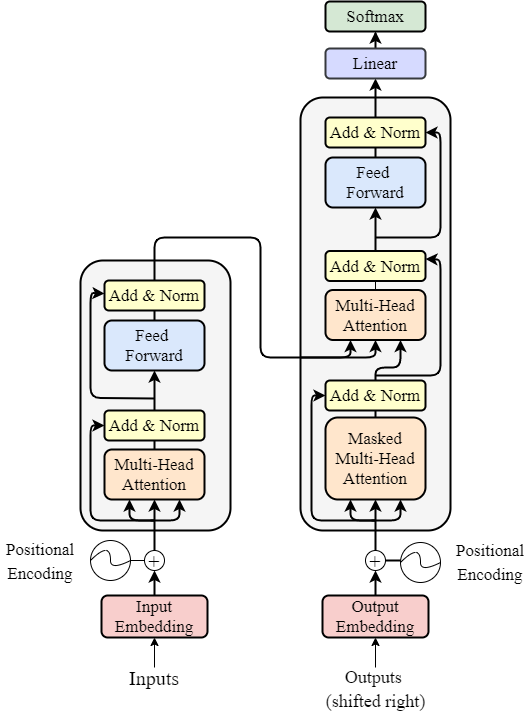
\includegraphics[scale=0.5]{images/fig_chapter2/nns/transformer_arch.png}
    \caption{Transformer Architecture}
    \label{fig:transformer_arch}
\end{figure}

\begin{figure}[H]
    \centering
    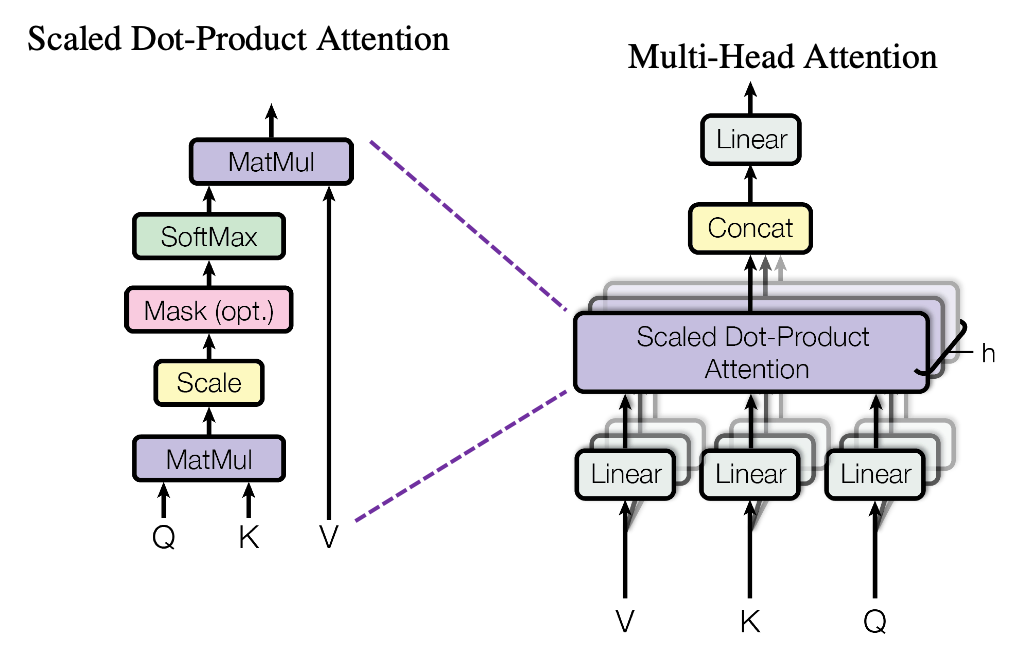
\includegraphics[scale=0.4]{images/fig_chapter2/nns/mha_img_original.png}
    \caption{Multi Headed Attention}
    \label{fig:mha}
\end{figure}

% \begin{figure}[H]
%     \centering
%     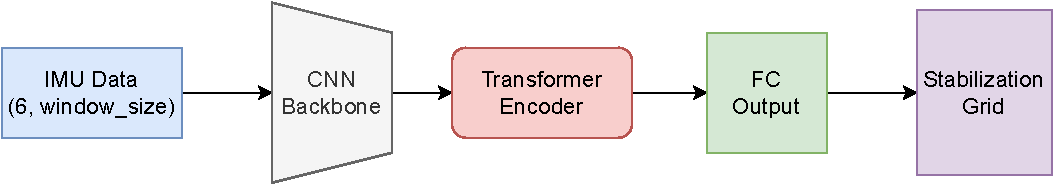
\includegraphics[scale=0.7]{images/fig_chapter2/nns/transformer_cnn.pdf}
%     \caption{CNN-Transformer}
%     \label{fig:transformer_cnn}
% \end{figure}


In this chapter we discussed different methods for image stabilization, challenges of pose-estimation and which methods are available to estimate pose from MEMS IMUs. The next chapter summaries some state of the art techniques used to solve the challenges we are facing.

% 3. Chapter: ''State of Research''
\chapter{State of Research} \label{chapter_three}

Previous chapter laid out the foundations for image stabilization and motion estimation. We also made the case for the techniques and algorithms chosen for this work. Now, this chapter includes some of the state-of-the-art methods for digital image stabilization and pose estimation. 

\section{Digital Image Stabilization}



\section{Pose Estimation}
\label{sec:sota_pose_est}
Classical algorithms fail to accurately estimate the pose using MEMS IMU over a long period of time. With the advancement of artificial neural networks (ANNs) and their architectures new data driven techniques have been developed for this purpose. These data-driven techniques have far outperformed their classical predecessors and are becoming a standard for this purpose. But with all these benefits they are computationally very expensive and have very high edge hardware requirements. 

\subsection{RIDI: Robust IMU Double Integration}
RIDI was the first data-driven neural network approach which tackles the challenges of double integrating accelerometer readings. The algorithm regresses a velocity vector from the history of linear accelerations and angular velocities (IMU windows - discussed in section \ref{sec:data_structure}), then corrects low-frequency bias in the linear accelerations, which are integrated twice to estimate position \citep{yan2018ridi}. The analysis of results manifested that this algorithm outperformed the heuristic-based methods and even came closer to visual inertial navigation \citep{yan2018ridi}. The issue with this is it can only regress position and orientation estimation needs to be achieved using classical algorithms.

\subsection{RoNIN: Robust Neural Inertial Navigation in the Wild}
Developed by the same team as RIDI, RoNIN uses more advanced neural network architectures like ResNet, LSTM and TCN as its backbone to regress a velocity vecotor given a window of IMU samples \citep{herath2020ronin}. Using these architectures and increasing the quality and size of data RoNIN outperforms RIDI and sets a new benchmark for inertial navigation. Our methodology is hugely infleuenced by this technique and is discussed in chapter \ref{chapter_four} of this report.

\subsection{TLIO: Tightly Learned Inertial Odometry}
This combines both classical and learn-based approaches by using an Extended Kalman Filter (EKF) and deep neural network (DNN). EKF is responsible for prediction step while outputs (displacement and uncertainty) from the neural network is used as measurement update. The filter estimates rotation, velocity, position and IMU biases at IMU rate \citep{hol2009tightly}. We could not reproduce the same results as the research claimed using our datasets.

\subsection{CTIN: Robust Contextual Transformer Network for Inertial Navigation}
This algorithm takes advantage of the recent advances in deep learning by using Multi-Headed-Attention (MHA) mechanism introduced in \citep{vaswani2017attention}. It uses a ResNet based encoder enhanced by local and global MHA to capture spatial contextual information from IMU measurements \citep{rao2022ctin}. CTIN is claimed to be robust and to outperform state-of-the-art models but cannot be evaluated as it is not available publicly.




% 4. Chapter: ''Methods''
\chapter{Work Methodology} \label{chapter_four}

We will be using an IMU sensor for camera pose estimation to stabilize the video for this work. Based on the precision requirements of the pose-estimation algorithm we will be using a data-driven approach as classical signal processing and sensor fusion algorithms fail to provide this precision over a long period of time. For our data driven approach we build datasets using a camera and also simulation. To capture the video we are using a GoPro Hero 10 which provides synchronised image and sensor data capture. We also swapped the factory lens to a low Field of View (FOV) and high focal length lens. The simulation was build using Unreal Engine 4 and Microsoft AirSim. Table \ref{tab:technical_details} shows the technical specifications of the camera setup. For simulation similar camera parameters were used.

\begin{table}
    \centering
\begin{tabular}{ c| c | L }

     Image Sensor & 
     Sony & 
     Diagonal 7.85 mm (Type 1/2.3) 23.91 M CMOS Image Sensor with Square Pixel. \\
     \hline
     
     IMU Sensor & 
     Bosch & 
     6-axis IMU Sensor
     Accelerometer (A): 16-bit or 0.06 mg/LSB 
     Gyroscope (G): 16-bit or 0.004 dps/LSB  \\
     \hline
     
     Lens & 
     xx & 
     15° FOV and 00 mm focal length \\

\end{tabular}
    \caption{Technical Specification}
    \label{tab:technical_details}
\end{table}

\section{Data Collection}
Collecting data for any data driven approach is a challenging and an iterative process. The data or training data in this case are the readings coming from the IMU sensor and the target (ground truth) being the camera pose (position and orientation). Real data was collected by mounting the camera on a rig which had vibrations associated with it on movement. We made sure that the data depicts real life scenarios by moving the rig around in many different ways and let it vibrate and collect the data. The ground truth was generated using proprietary Zeiss software and is beyond the scope of this work. 

Then the data was collected from simulation based on the analysed real data and pushed beyond real data limits to account for even more challenging scenarios. Generating simulated data with accurate ground truth is a fast processes not requiring much post-processing. This also allowed us to tinker with noise and bias to make the neural network robust and generalize well.

\subsection{Data Analysis}
\label{data_analysis}
The data recorded from a camera-rig setup was analysed to determine the vibration and sensor parameters. Table \ref{tab:imu_noise_characteristics} summarises the white noise and bias characteristics determined from the raw IMU Sensor Readings. These match closely with the data provided by the manufacturer. Accelerometer variance from data sheet $ 160 \mu g /\sqrt{Hz} $ and for gyroscope $ 0.008 dps /\sqrt{Hz}  $.

\begin{table}[ht]
\centering
\begin{tabular}{l|c}
    Parameter & Value \\ \hline
    Accelerometer Bias & xx \\  
    Accelerometer White Noise & $ \mu = 0 $ and $ \sigma^{2}=0.xxx $ \\  
    Gyro Bias & xx \\  
    Gyro White Noise & $ \mu = 0 $ and $ \sigma^{2}=0.xxx $ \\  
\end{tabular}
\caption{IMU Noise Characteristics}
\label{tab:imu_noise_characteristics}
\end{table}

We analysed the generated ground truth to determine the characteristics of vibration. These characteristics are important to understand the nature of vibration and to set the working limits for our work. Vibrations are characterised by \textbf{Amplitude} ( A or  $ \theta $), \textbf{Time Constant} ($ \tau $) and \textbf{Frequency} ($ \omega $). We have damped oscillations for both displacement and rotation vibration as shown in figure \ref{fig:damped_vib} and can be characterised by the equations \ref{eqn:vib_disp} and \ref{eqn:vib_rot}.

\begin{figure}
    \centering
    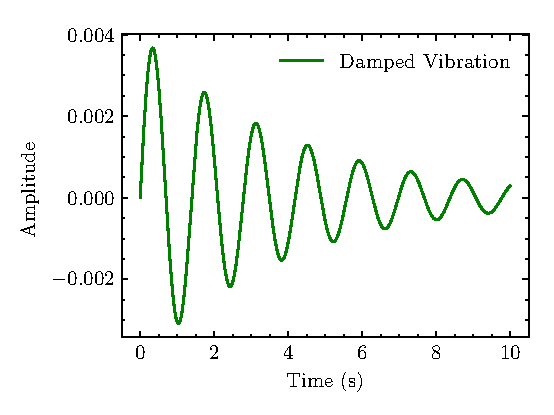
\includegraphics{images/fig_chapter4/vib_damped.eps}
    \caption{Damped Vibration}
    \label{fig:damped_vib}
\end{figure}

\begin{equation}
  \label{eqn:vib_disp}
  \begin{aligned}
    A(t) = Ae^{-t/\tau}sin(2\pi\omega t) \\
  \end{aligned}
\end{equation}

\begin{equation}
  \label{eqn:vib_rot}
  \begin{aligned}
    \theta(t) = \theta e^{-t/\tau}sin(2\pi\omega t) \\
  \end{aligned}
\end{equation}

%% Displacement distribution
\begin{figure}
    %%
    \begin{subfigure}{\linewidth}
    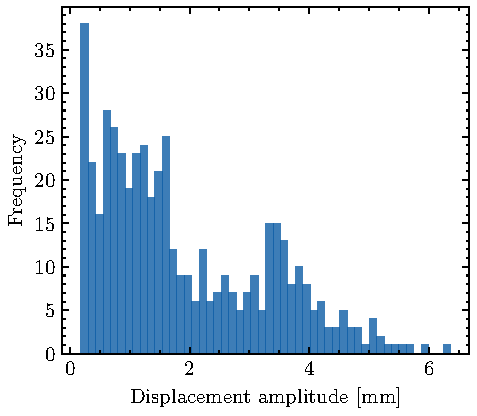
\includegraphics[width=.5\linewidth]{images/fig_chapter4/data_dist/1.pdf}\hfill
    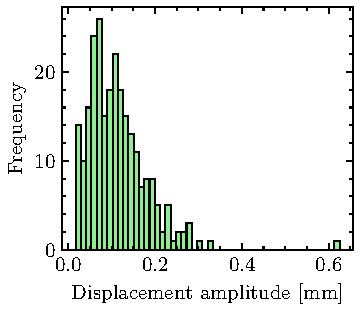
\includegraphics[width=.5\linewidth]{images/fig_chapter4/data_dist/2.pdf}
    \caption{Distribution of displacement amplitude $ A $ in XY(left) and Z(right) DoF [mm]}
    \end{subfigure}\par\medskip
    
    %%
    \begin{subfigure}{\linewidth}
    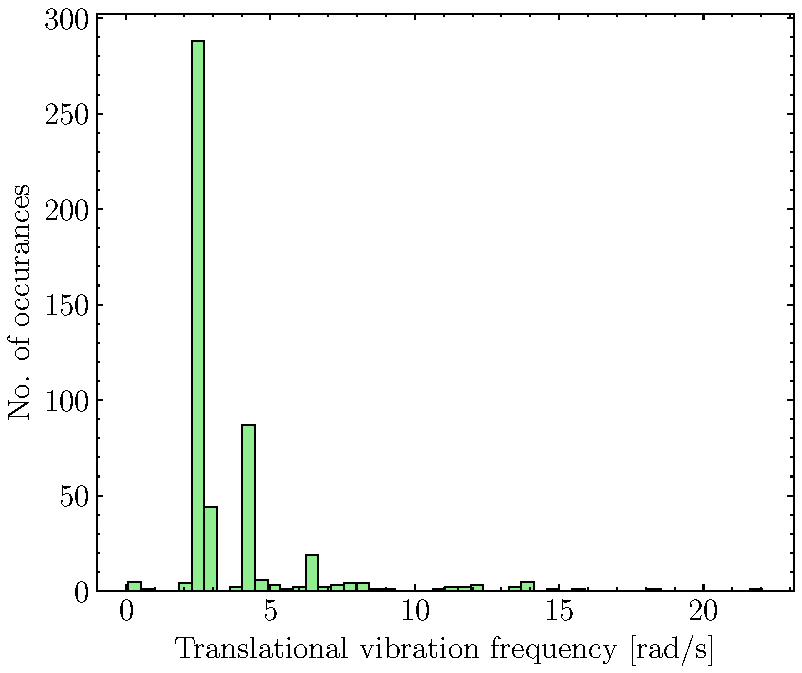
\includegraphics[width=.5\linewidth]{images/fig_chapter4/data_dist/3.pdf}\hfill
    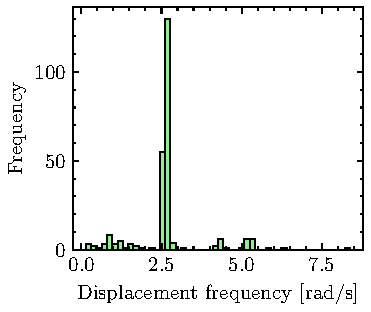
\includegraphics[width=.5\linewidth]{images/fig_chapter4/data_dist/4.pdf}
    \caption{Distribution of displacement frequency $ \omega $ in XY(left) and Z(right) DoF [mm]}
    \end{subfigure}\par\medskip
    
    %%
    \begin{subfigure}{\linewidth}
    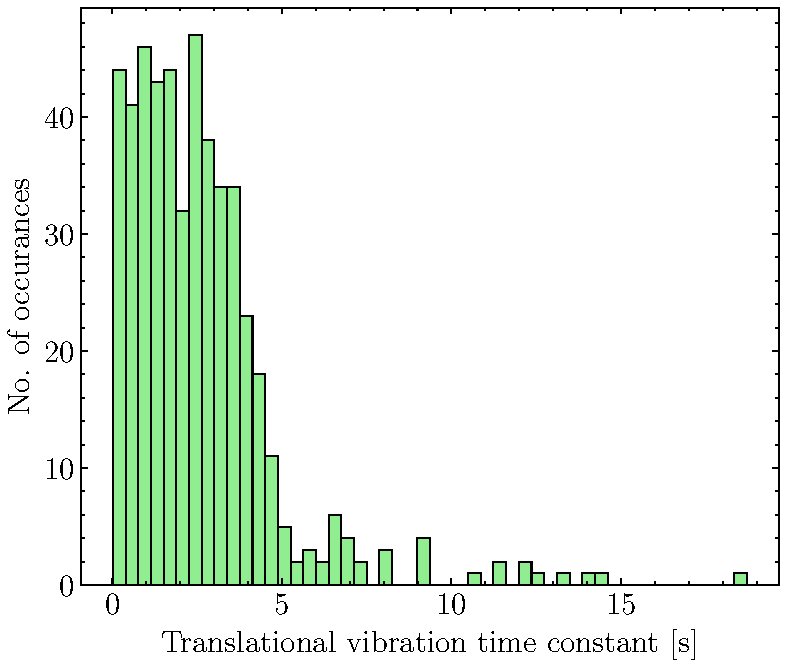
\includegraphics[width=.5\linewidth]{images/fig_chapter4/data_dist/5.pdf}\hfill
    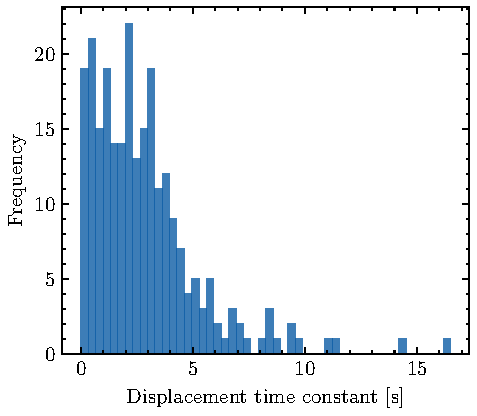
\includegraphics[width=.5\linewidth]{images/fig_chapter4/data_dist/6.pdf}
    \caption{Distribution of displacement time-constant $ \tau $ in XY(left) and Z(right) DoF [mm]}
    \end{subfigure}
\caption{Real displacement data statistical analysis}
\label{fig:dist_disp}
\end{figure}

%% Rotation Distribution 
\begin{figure}
    %%
    \begin{subfigure}{\linewidth}
    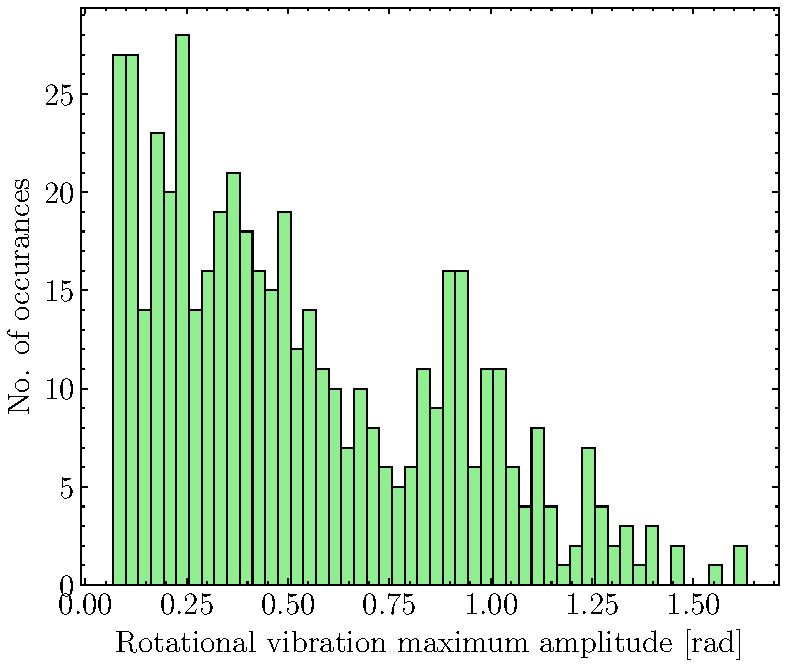
\includegraphics[width=.5\linewidth]{images/fig_chapter4/data_dist/7.pdf}\hfill
    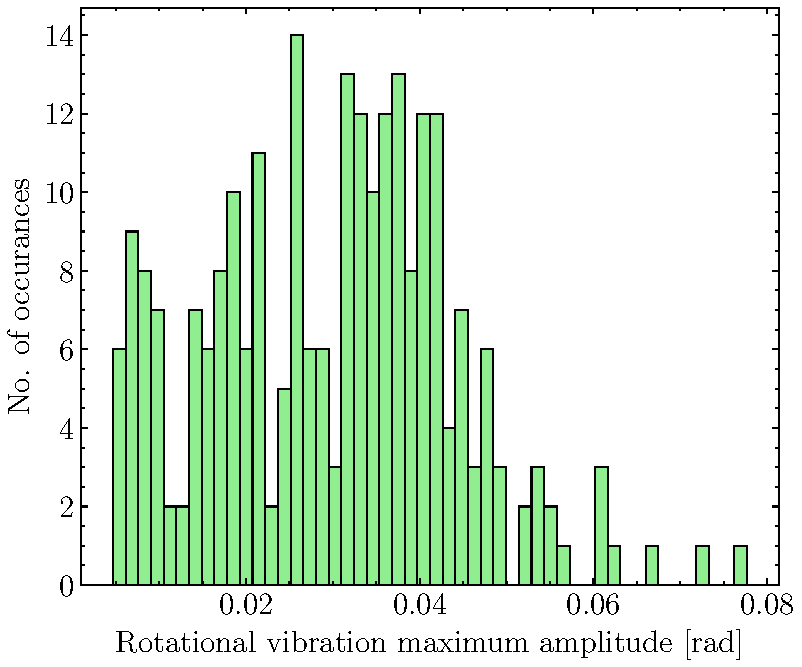
\includegraphics[width=.5\linewidth]{images/fig_chapter4/data_dist/8.pdf}
    \caption{Distribution of rotation amplitude $ \theta $ in XY(left) and Z(right) DoF [mm]}
    \end{subfigure}\par\medskip
    
    %%
    \begin{subfigure}{\linewidth}
    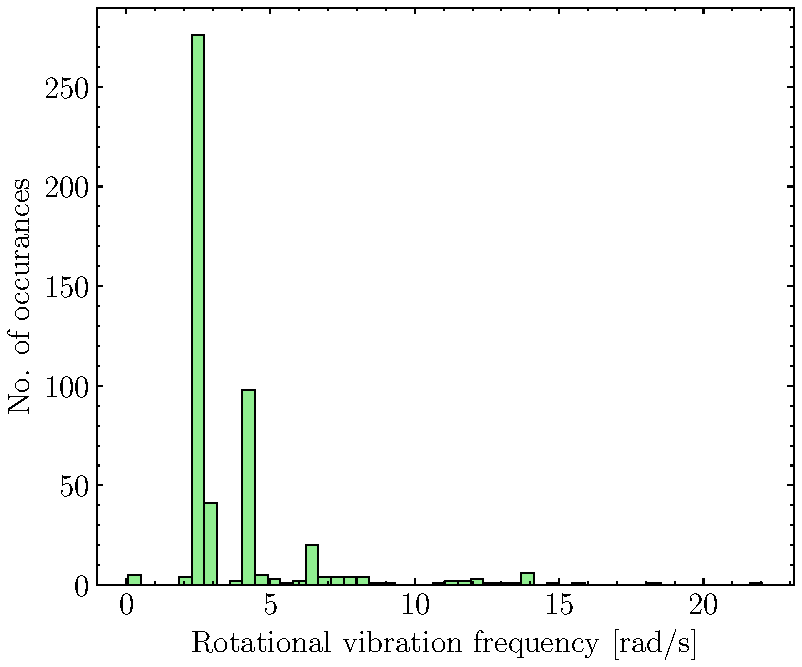
\includegraphics[width=.5\linewidth]{images/fig_chapter4/data_dist/9.pdf}\hfill
    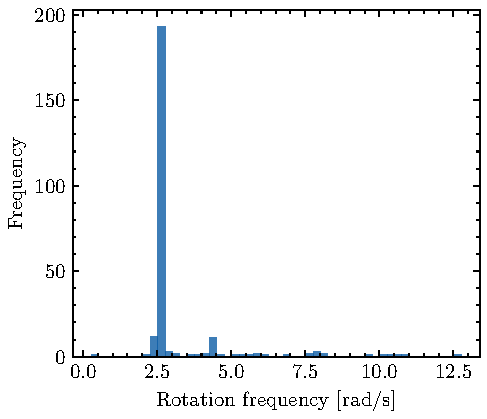
\includegraphics[width=.5\linewidth]{images/fig_chapter4/data_dist/10.pdf}
    \caption{Distribution of rotation frequency $ \omega $ in XY(left) and Z(right) DoF [mm]}
    \end{subfigure}\par\medskip
    
    %%
    \begin{subfigure}{\linewidth}
    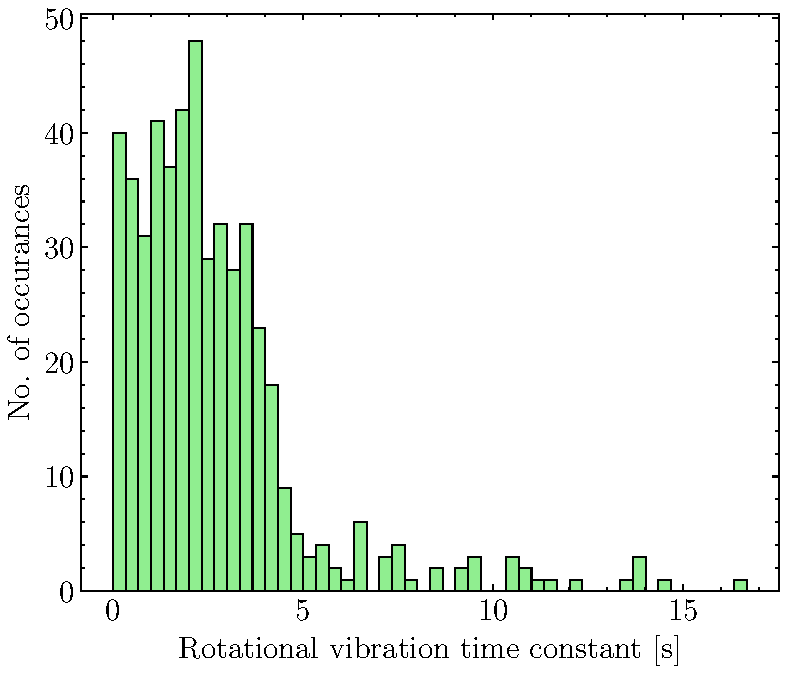
\includegraphics[width=.5\linewidth]{images/fig_chapter4/data_dist/11.pdf}\hfill
    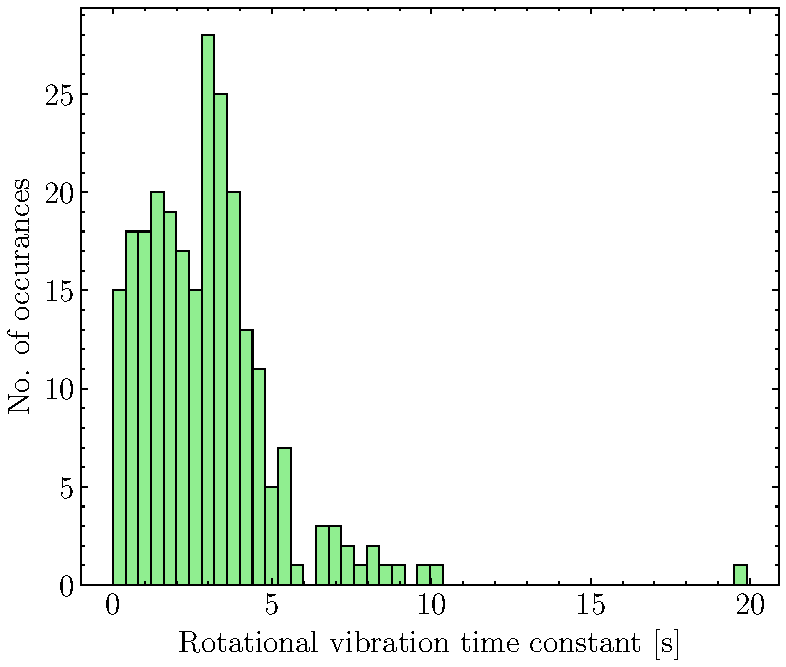
\includegraphics[width=.5\linewidth]{images/fig_chapter4/data_dist/12.pdf}
    \caption{Distribution of rotation time-constant $ \tau $ in XY(left) and Z(right) DoF [mm]}
    \end{subfigure}

\caption{Real rotation data statistical analysis}
\label{fig:dist_rot}
\end{figure}


The statistical analysis shown in figure \ref{fig:dist_disp} and figure \ref{fig:dist_rot} was done on 248 vibration sequences with an average length of 10 seconds. The results for displacement and rotation vibrations are summarised in table \ref{tab:real_data_analysis_displacement} and table \ref{tab:real_data_analysis_rotation} respectively. The rotational vibrations have very small amplitude ($ \theta $) and is less than 1 degrees for more than 75 percent of the samples in XY plane. For Z axis the vibrations are even smaller with a mean of 0.0005 degrees. These vibrations are very small and do not have a a noticeable visual effect on the video stabilization. But we have decided to account for them to develop a more general solution with multiple applications. The time constant ($ \tau $) for displacement and rotation is similar for all DoF with a mean value of around 2.9 seconds.  The frequency ($ \omega $) for all DoF is also similar in the range $ 2.5 rad/sec $ to $ 3.5 rad/sec $. Frequency of $ 2.5 rad/sec $ is the most dominant frequency and seems to be the natural frequency $ \omega_n $ of the mechanical system (rig on which the camera is mounted).


The amplitude ($ A $) of the vibration displacement is the most important characteristic for this work as it is main source of video destabilization. The effect of motion on the quality of video is more pronounced in XY plane as the most pixel shift happens here. In Z axis the mean ($ \mu $) of vibrations is 0.113 mm with a standard deviation ($ \sigma^{2} $) of 0.07 mm. Even the large vibrations in Z seem to have little effect on visual quality of the video. Vibrations in XY plane have the mean of 1.9 mm with a standard deviation of 1.36 mm. Vibrations with higher magnitude are also present and need to be accounted for when generating simulated data.




% displacement data distribution table
\begin{table}[ht]
    \centering
\begin{tabular}{ c | L | L | L }
    
     Parameter  & 
     Mean ($ \mu $) & 
     Variance ($ \sigma^{2} $) &
     Standard Deviation ($ \sigma $)\\
     \hline
     
     $ A_{xy} $ & 
     $ 1.8944 mm $ & 
     $ 1.8674 mm^{2} $ &
     $ 1.3665 mm $ \\

      
     $ A_{z} $  & 
     $ 0.1135 mm $ & 
     $ 0.0047 mm^{2} $ &
     $ 0.0690 mm $ \\
     
     
     $ \omega_{xy} $ & 
     $ 3.6898 rad/s $ & 
     $ 5.9833 rad^{2}/s^{2} $ &
     $ 2.4460 rad/s $ \\
     
     
     $ \omega_{z} $& 
     $ 2.6835 rad/s $ & 
     $ 2.0765 rad^{2}/s^{2} $ &
     $ 1.0375 rad/s $ \\

     
     $ \tau_{xy} $ & 
     $ 2.5914 s $ & 
     $ 5.1898 s^{2} $ &
     $ 2.2781 s $ \\


     $ \tau_{z} $ & 
     $ 2.8396 s $ & 
     $ 5.8720 s^{2} $ &
     $ 2.4243 s $ \\

\end{tabular}
    \caption{Real Data displacement-vibration distributions}
    \label{tab:real_data_analysis_displacement}
\end{table}

% rotation data distribution table
\begin{table}[ht]
    \centering
\begin{tabular}{ c | L | L | L }

     Parameter  & 
     Mean ($ \mu $) & 
     Variance ($ \sigma^{2} $) &
     Standard Deviation ($ \sigma $)\\
     \hline
     
     $ \theta_{xy} $ & 
     $ 0.0094 rad $ & 
     $ 3.8729e^{-8} rad^{2} $ &
     $ 0.0062 rad $ \\

      
     $ \theta_{z} $  & 
     $ 0.0005 rad $ & 
     $ 6.0739e^{-8} rad^{2} $ &
     $ 0.0002 rad $ \\
     
     
     $ \omega_{xy} $ & 
     $ 3.8042 rad/s $ & 
     $ 6.3685 rad^{2}/s^{2} $ &
     $ 2.5236 rad/s $ \\

     
     $ \omega_{z} $& 
     $ 3.1763 rad/s $ & 
     $ 2.6238 rad^{2}/s^{2} $ &
     $ 1.6198 rad/s $ \\
   
     
     $ \tau_{xy} $ & 
     $ 2.6581 s $ & 
     $ 5.8362 s^{2} $ &
     $ 2.4158 s $ \\
    
     
     $ \tau_{z} $ & 
     $ 2.9316 s $ & 
     $ 4.7336 s^{2} $ &
     $ 2.1757 s $ \\

\end{tabular}
    \caption{Real Data rotational-vibration distributions}
    \label{tab:real_data_analysis_rotation}
\end{table}



\subsection{Simulated Data Generation}
\label{sec:gen_sim_data}
The simulated data plays a very important role in our approach as we use the ideal data to validate our stabilization approach. It also empowers us to simulate IMU sensors with different noise levels and characteristics. We also made sure that the data generated from the simulation is fairly domain randomized to make it realistic. 

Simulated data is based on the analysed real data with vibration characteristics taken from table \ref{tab:real_data_analysis_displacement} and table \ref{tab:real_data_analysis_rotation}. The data is then generated using the equations \ref{eqn:vib_disp} and \ref{eqn:vib_rot} .The simulated data is then augmented with modified noise and bias characteristics from table \ref{tab:imu_noise_characteristics}. A total of 600 vibration sequences with an average vibration duration of 15 seconds was generated with characteristics shown in tables \ref{tab:real_data_analysis_displacement} and \ref{tab:real_data_analysis_rotation}. Generating a large number of samples ensures the sampling of diverse data from the distribution. This is where we benefit from our simulation the most as the diversity and the size of data ensures our neural network generalizes well.



% Sim Vibration characteristics
 \begin{table}[ht]
\centering
\begin{tabular}{ c | L | L | L }
    
     Parameter  & 
     Mean ($ \mu $) & 
     Variance ($ \sigma^{2} $) &
     Standard Deviation ($ \sigma $)\\
     \hline
     
     $ A_{xy} $ & 
     $ 2.5 mm $ & 
     $ 2.2 mm^{2} $ &
     $ 1.48 mm $ \\

      
     $ A_{z} $  & 
     $ 0.4 mm $ & 
     $ 0.01 mm^{2} $ &
     $ 0.1 mm $ \\
     
     
     $ \omega_{xy} $ & 
     $ 4.5 rad/s $ & 
     $ 6.5 rad^{2}/s^{2} $ &
     $ 2.55 rad/s $ \\
     
     
     $ \omega_{z} $& 
     $ 3.5 rad/s $ & 
     $ 2.5 rad^{2}/s^{2} $ &
     $ 1.58 rad/s $ \\

     
     $ \tau_{xy} $ & 
     $ 3.5 s $ & 
     $ 6.0 s^{2} $ &
     $ 2.45 s $ \\


     $ \tau_{z} $ & 
     $ 3.5 s $ & 
     $ 6.0 s^{2} $ &
     $ 2.45 s $ \\
    
    \hline
    \hline
    
     $ \theta_{xy} $ & 
     $ 0.001 rad $ & 
     $ 5e^{-7} rad^{2} $ &
     $ 7.1^{-4} rad $ \\

      
     $ \theta_{z} $  & 
     $ 0.001 rad $ & 
     $ 6e^{-7} rad^{2} $ &
     $ 7.75^{-4} rad $ \\
     
     
     $ \omega_{xy} $ & 
     $ 4.5 rad/s $ & 
     $ 7 rad^{2}/s^{2} $ &
     $ 2.65 rad/s $ \\

     
     $ \omega_{z} $& 
     $ 4 rad/s $ & 
     $ 3 rad^{2}/s^{2} $ &
     $ 1.73 rad/s $ \\
   
     
     $ \tau_{xy} $ & 
     $ 3 s $ & 
     $ 6.2 s^{2} $ &
     $ 2.5 s $ \\
    
     
     $ \tau_{z} $ & 
     $ 3.3 s $ & 
     $ 5 s^{2} $ &
     $ 2.24 s $ \\
     
\end{tabular}
    \caption{Simulated vibration data characteristics}
    \label{tab:sim_vib_characteristics}
\end{table} %%%%


\section{Structuring of Data}
\label{sec:data_structure}
In classical pose-estimation techniques, every single IMU sample is used individually along with initial condition. Data driven approaches differ in this case as discussed in section \ref{sec:sota_pose_est}. For data driven approaches instead of taking an individual sample a \textit{window} of samples (figure \ref{fig:imu_window_samples})is used as a single sample does not contain enough information. Neural Networks unlike classical mathematics based approaches are data hungry and look for patterns in data and based on these patterns they generate an output. Initially we experimented with small window samples (3 - 20 samples) as shown in figure \ref{fig:imu_window_samples} a. This did not yield very good results and the pose estimation error was higher than the required. It started giving good results once we reach a IMU \textbf{ window size} of 70 to 140 samples (figure \ref{fig:imu_window_samples}). Beyond these the performance does not improve much and the inferences from the neural network become computationally expensive and inference latency become very high.

%% Displacement distribution
\begin{figure}
    %%
    \begin{subfigure}{\linewidth}
    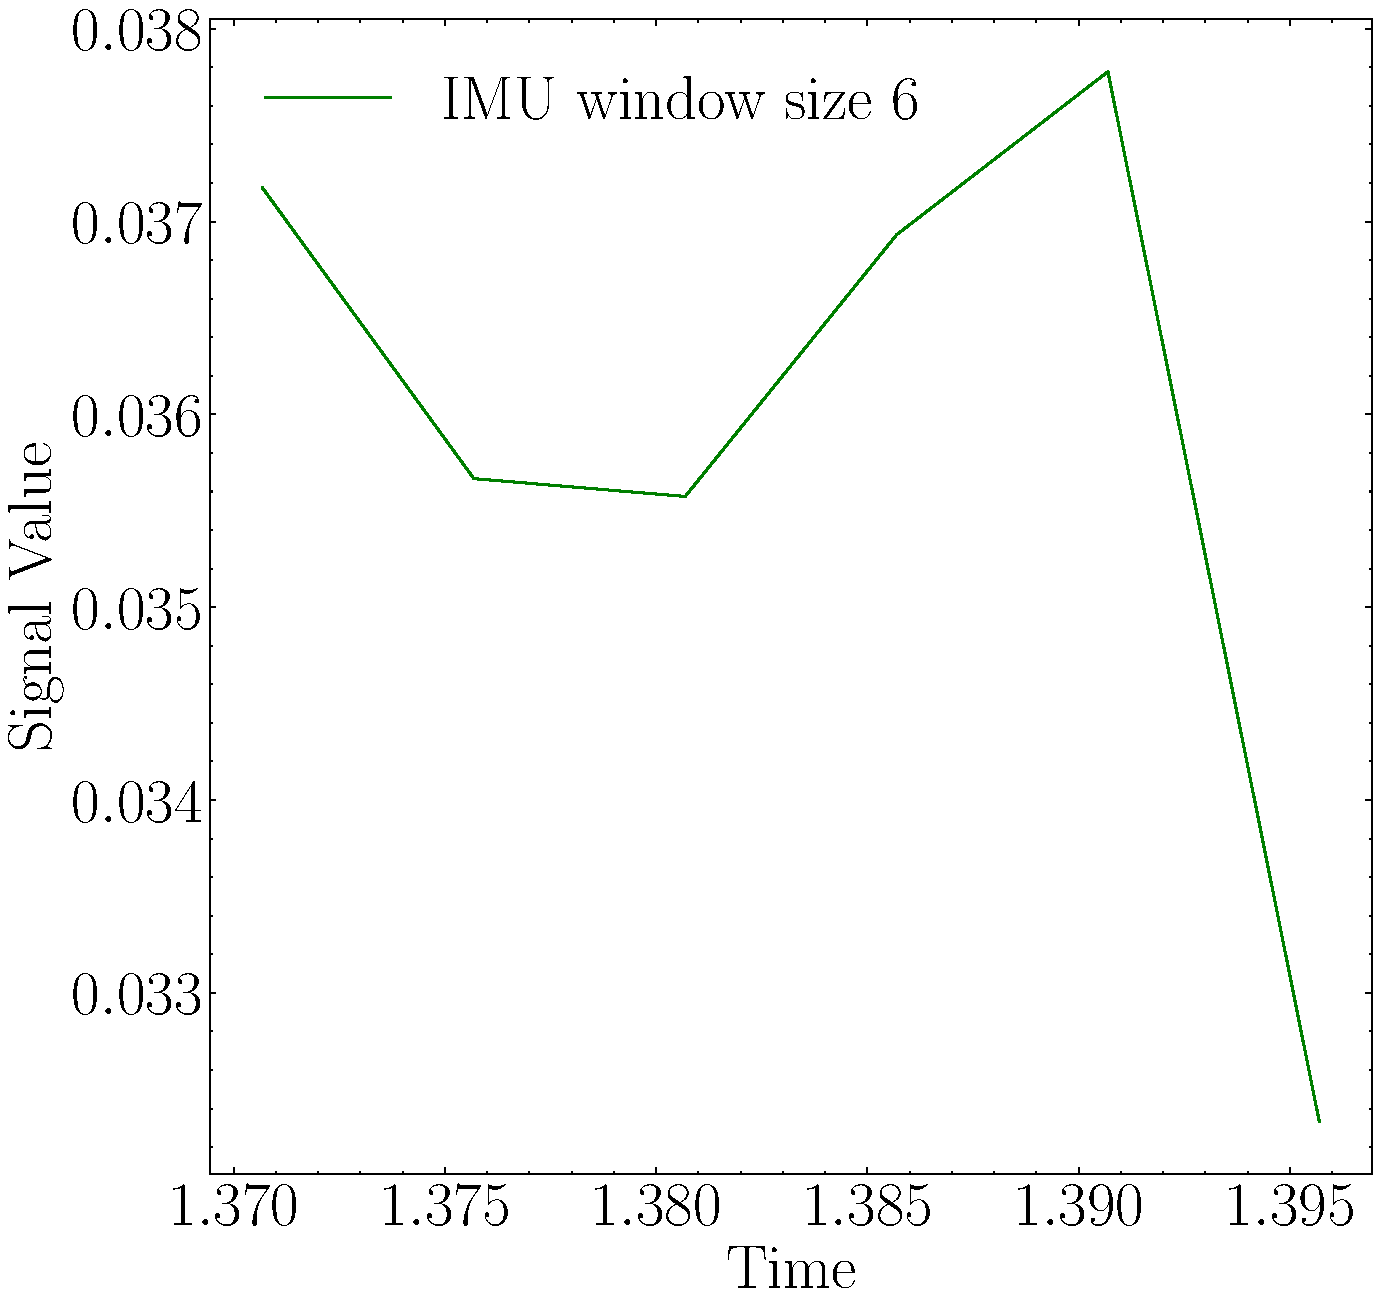
\includegraphics[width=.3\linewidth]{images/fig_chapter4/imu_windows/imu_window_size_6.pdf}\hfill
    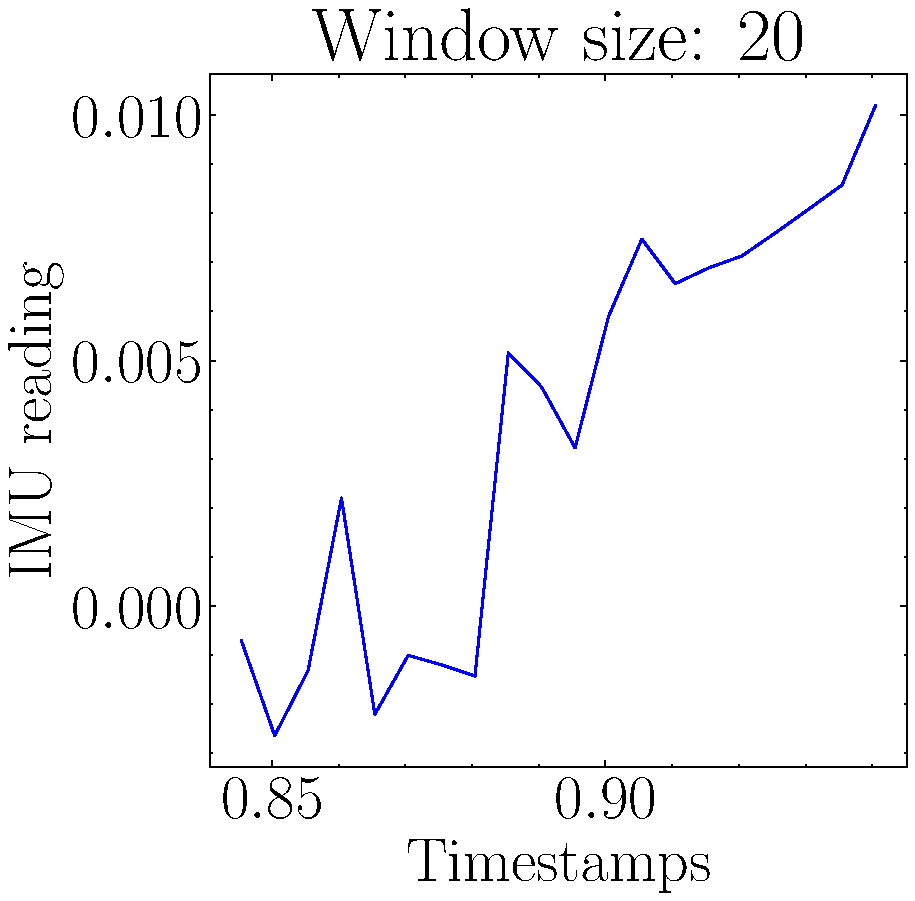
\includegraphics[width=.3\linewidth]{images/fig_chapter4/imu_windows/imu_window_size_20.pdf}\hfill
    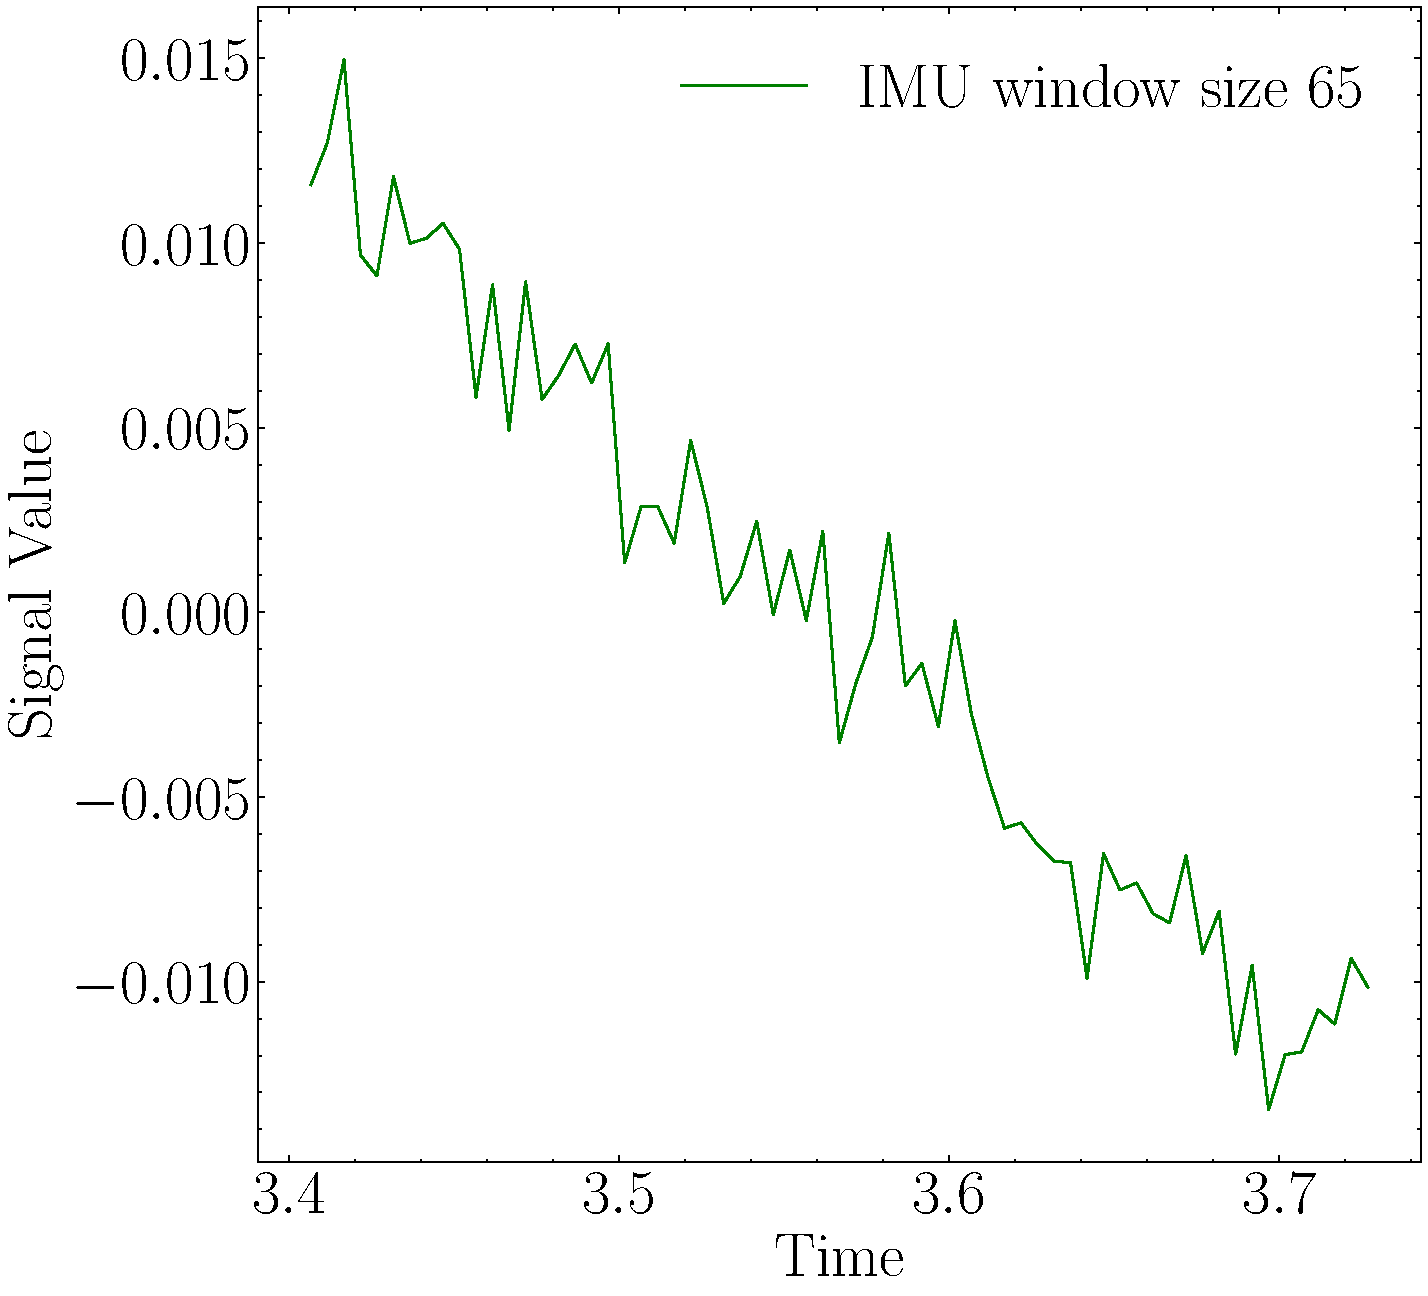
\includegraphics[width=.3\linewidth]{images/fig_chapter4/imu_windows/imu_window_size_65.pdf}\hfill
    \caption{Window size 6, 20 and 65}
    \end{subfigure}\par\medskip
    
    %%
    \begin{subfigure}{\linewidth}
    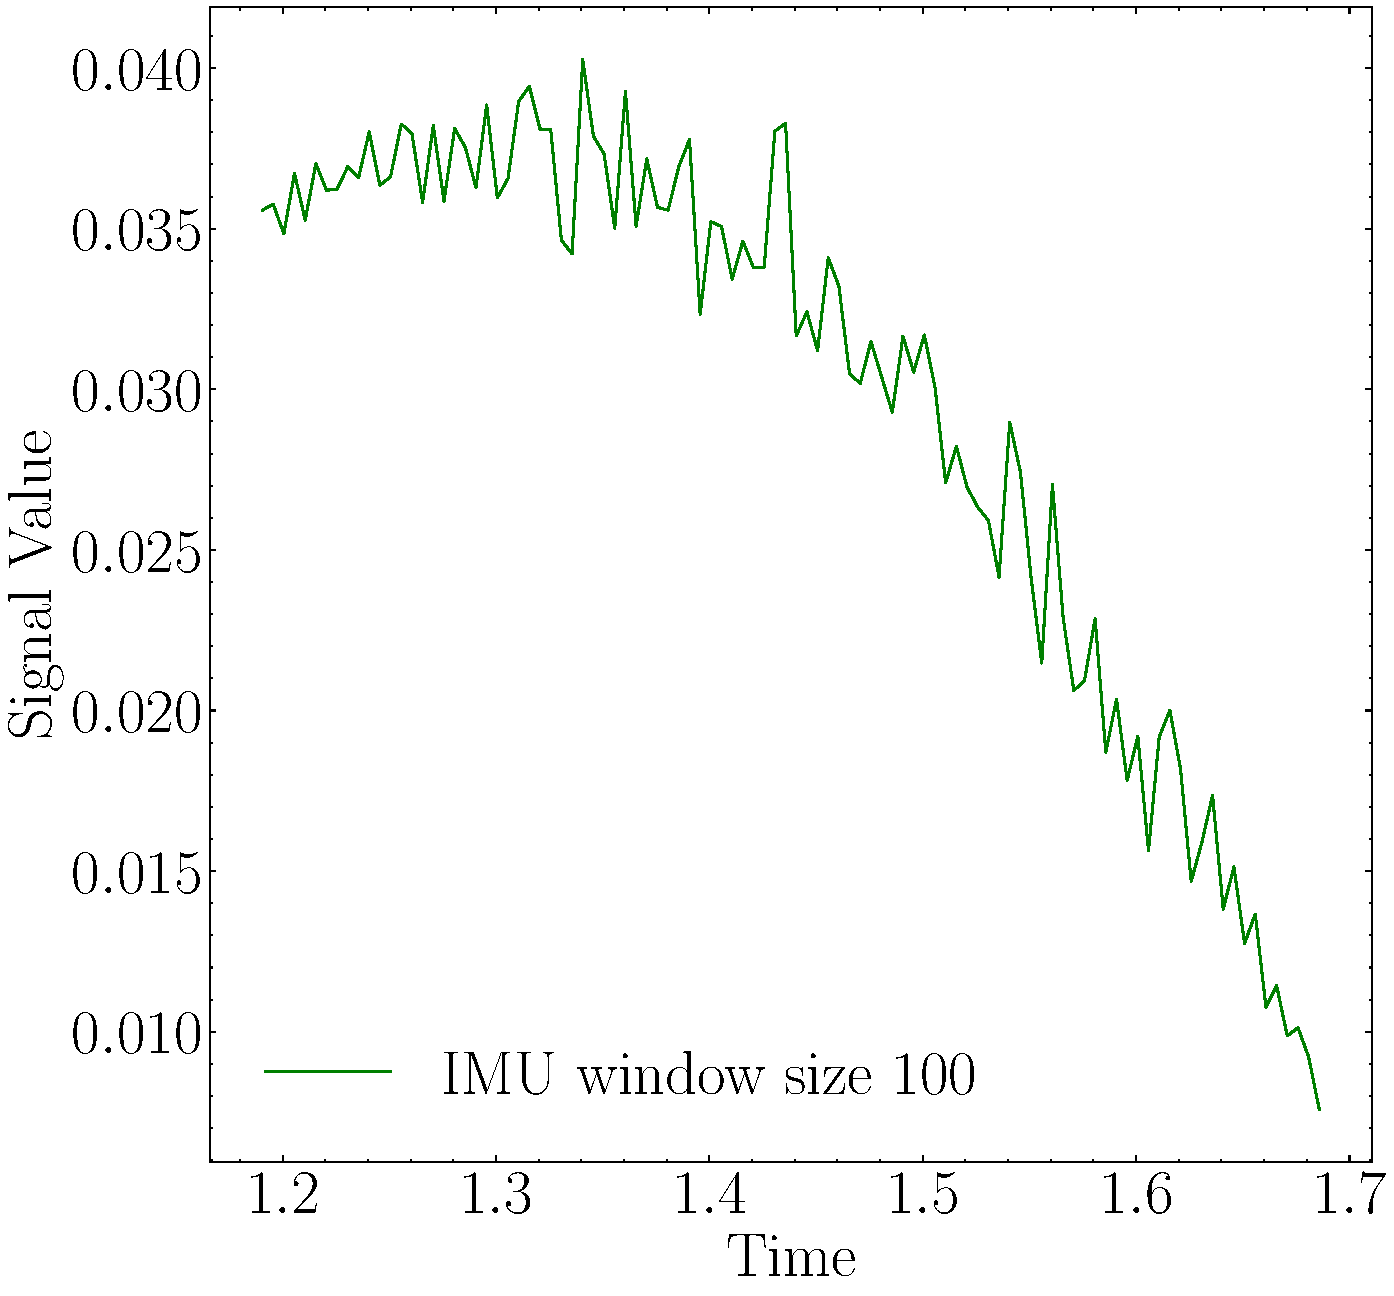
\includegraphics[width=.3\linewidth]{images/fig_chapter4/imu_windows/imu_window_size_100.pdf}\hfill
    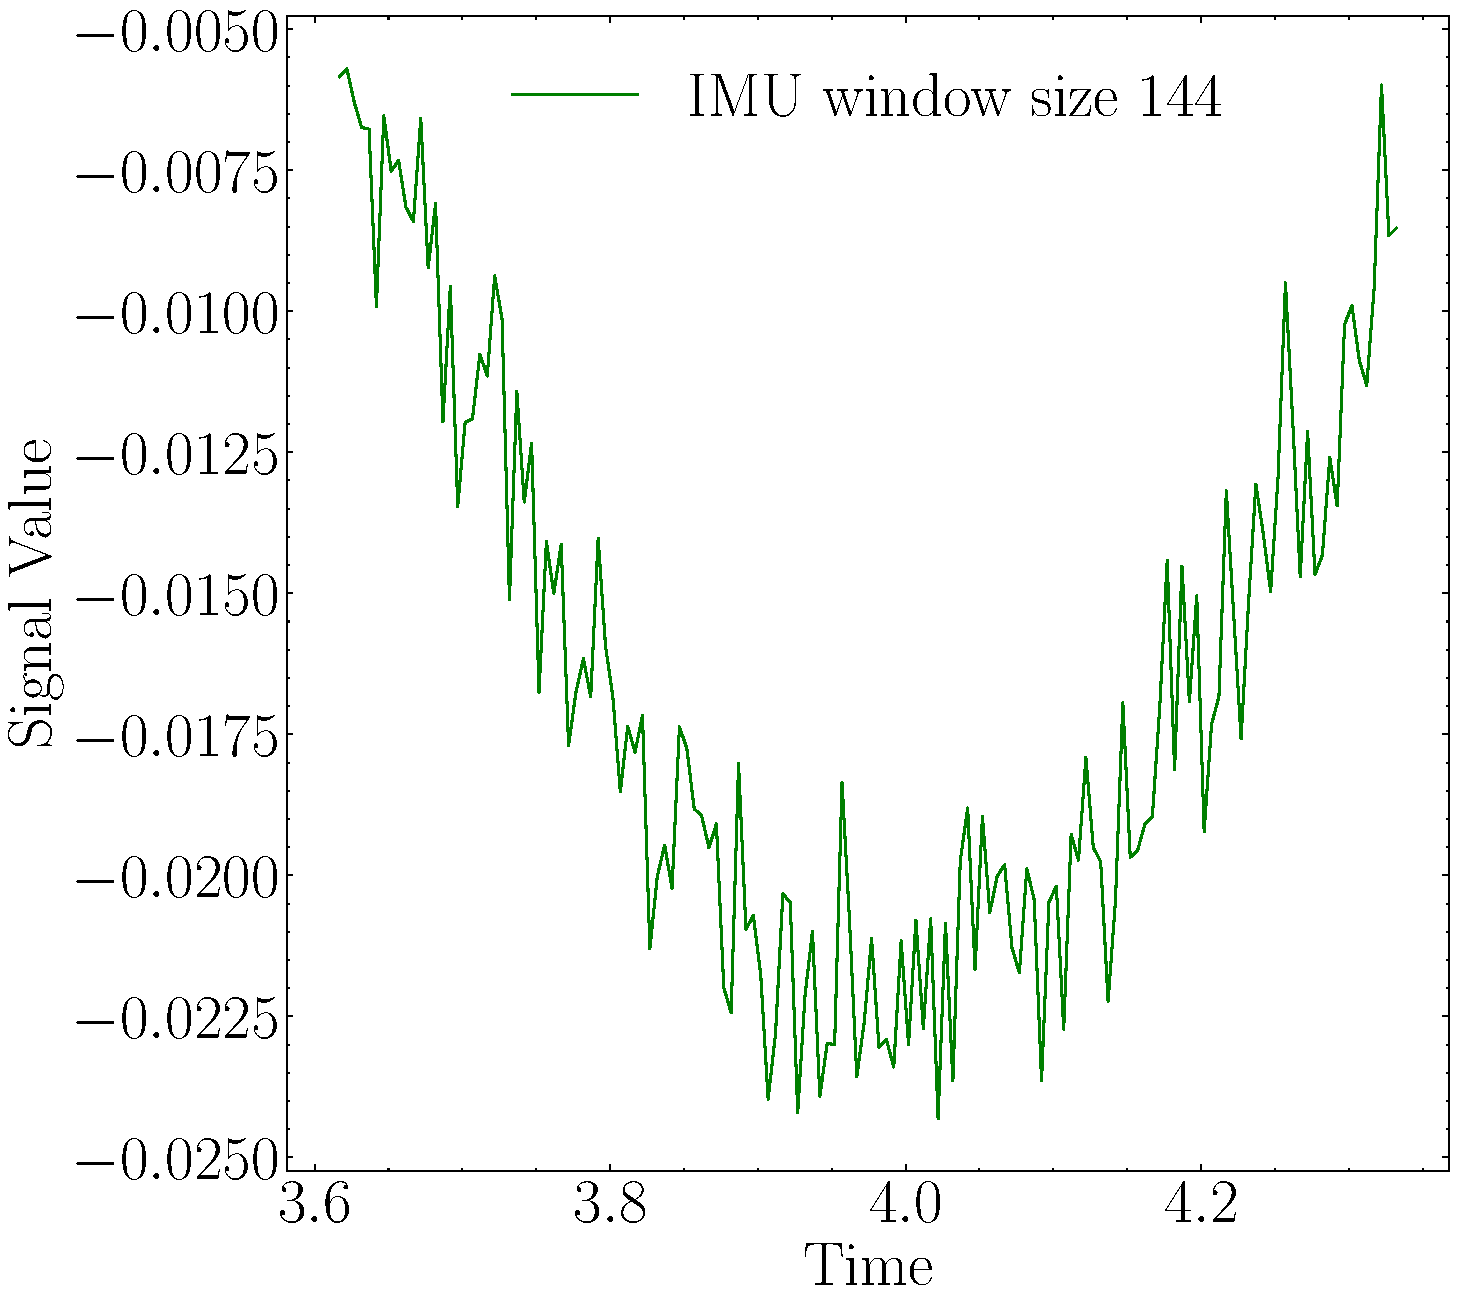
\includegraphics[width=.3\linewidth]{images/fig_chapter4/imu_windows/imu_window_size_144.pdf}\hfill
    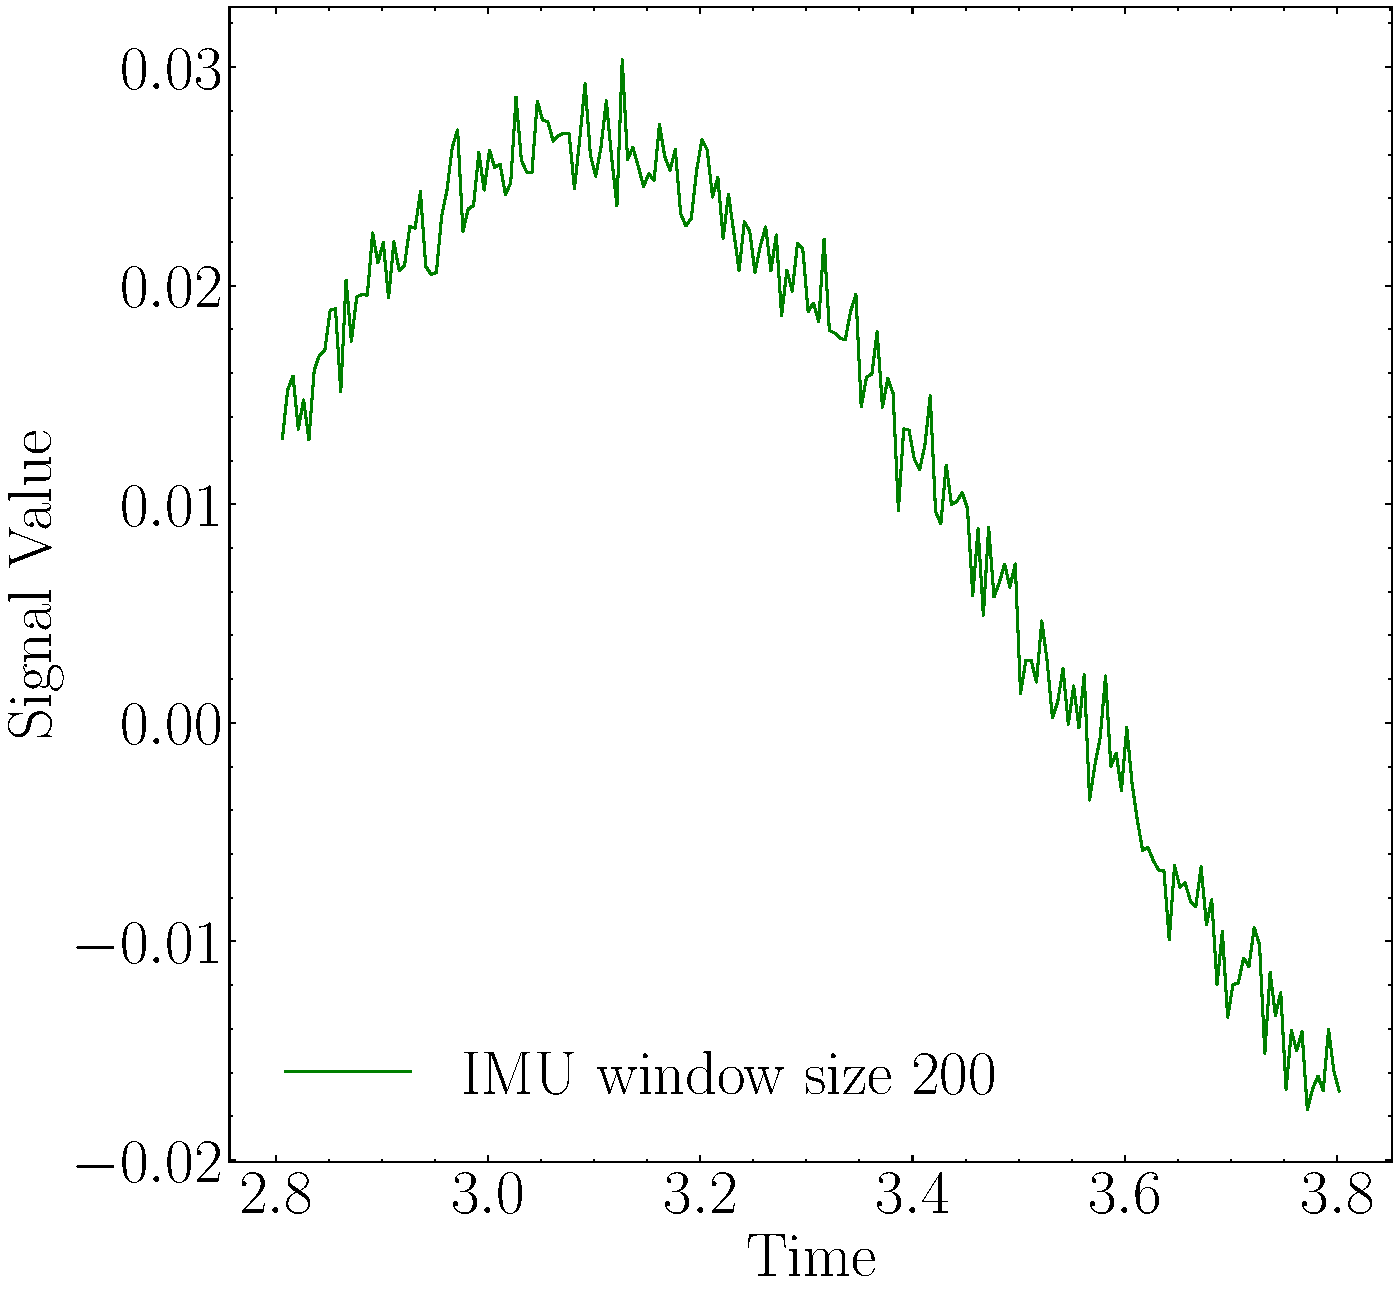
\includegraphics[width=.3\linewidth]{images/fig_chapter4/imu_windows/imu_window_size_200.pdf}\hfill
    \caption{Window size 100, 144, 200}
    \end{subfigure}
\caption{Different IMU window samples}
\label{fig:imu_window_samples}
\end{figure}


\section{Mathematics for stabilisation}
Here we will see what exactly we are trying to find out: (R, T)

\section{Training and Testing of Various Neural Networks}
Various neural networks architectures were trained and tested to accurately estimate the camera pose with respect to a stabilised trajectory. Network takes as input the sensor readings coming from an IMU and the network is trained against the deviation with respect to stabilization trajectory. The stabilization trajectory can be realised as a mean of the vibration displacement (linear/angular) for an ideal case as shown in figure \ref{fig:stab_traj_ideal}. 

\begin{figure}
    \centering
    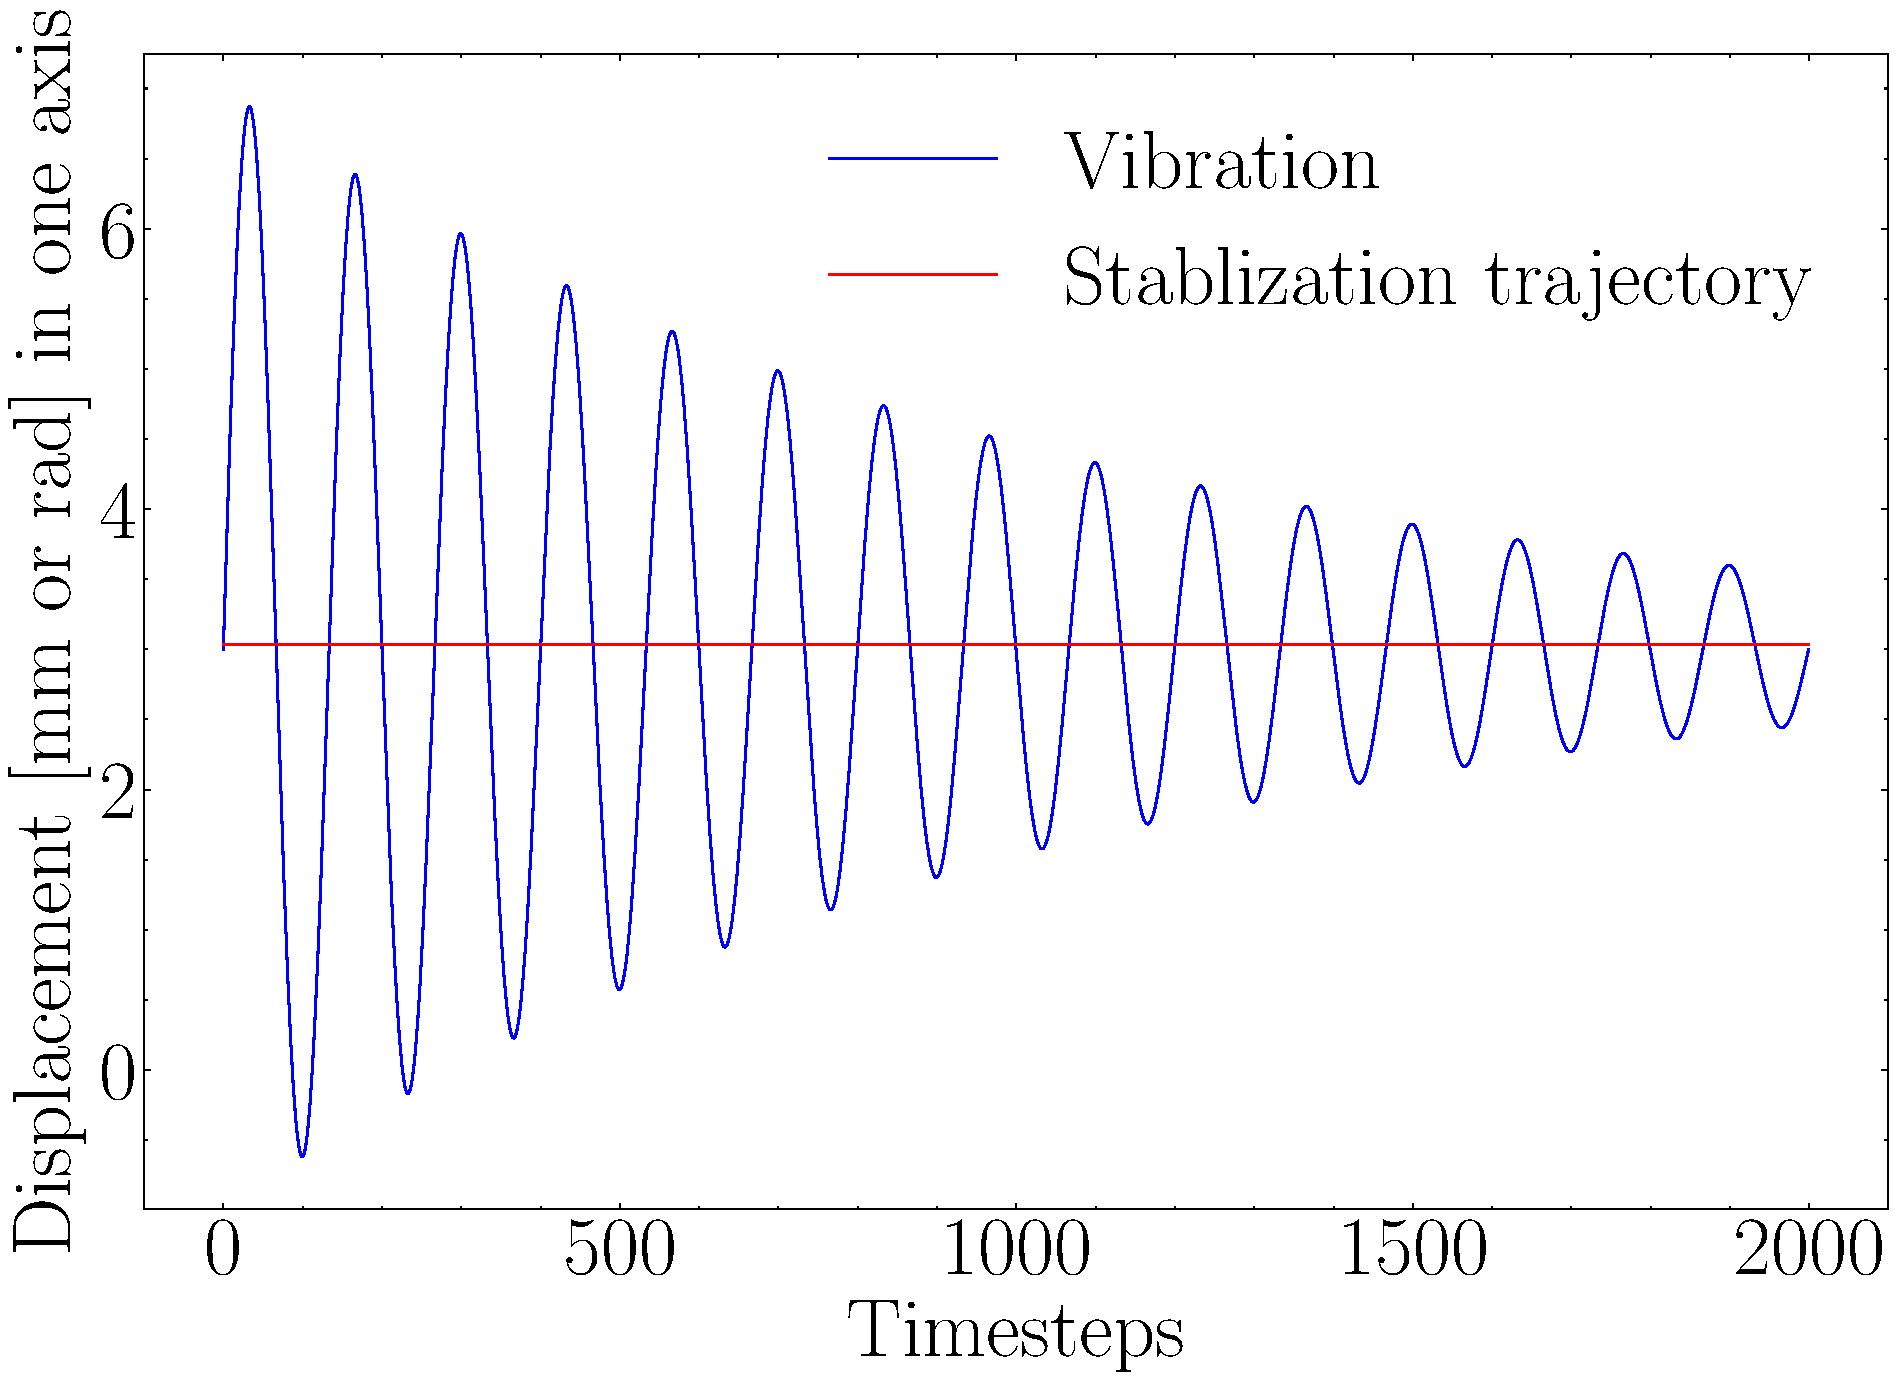
\includegraphics[scale=0.25]{images/fig_chapter2/stab_traj_ideal.pdf}
    \caption{Stabilization Trajectory (Ideal)}
    \label{fig:stab_traj_ideal}
\end{figure}

The size of input to the network is variable based on which if we want to only use Accelerometer readings (3, window-size) or both Accelerometer and Gyroscope sensor readings (6, window-size). The use of accelerometer readings is must because destabilization caused in our use case is mostly due to linear displacements as discussed in chapter section \ref{sec:imu} of this report. 

Various neural network architectures like CNN, MLP, LSTM, ResNet, Transformers and their variations were trained and tested for stabilization trajectory regression. Out of these CNN, ResNet and Transformer architectures had acceptable performance. 

\subsection{Convolutional Neural Network}
Convolution neural network with six \textbf{1D-Convolutional} Layers in sequence with \textbf{Batch Normalisation} and  \textbf{ReLU} activation is used to extract features from the input data. Then the output of these convolution layers is regularized using \textbf{dropout} and down-sampled using \textbf{Max-pooling}. Finally, pose is regressed using a series of two fully connected \textbf{Linear} layers.

\subsubsection{Model Output Analysis}
Figure xx shows the model output vs ground truth plot for a 27 seconds video in all 6 DoF (3 Linear and 3 Angular Displacement). The model can regress stabilization trajectory based on input IMU readings with good precision but there are zones where the prediction is off and thus causes jitter in stabilization. The error in all DoF can be seen in figure xx.


\begin{figure}
    \centering
    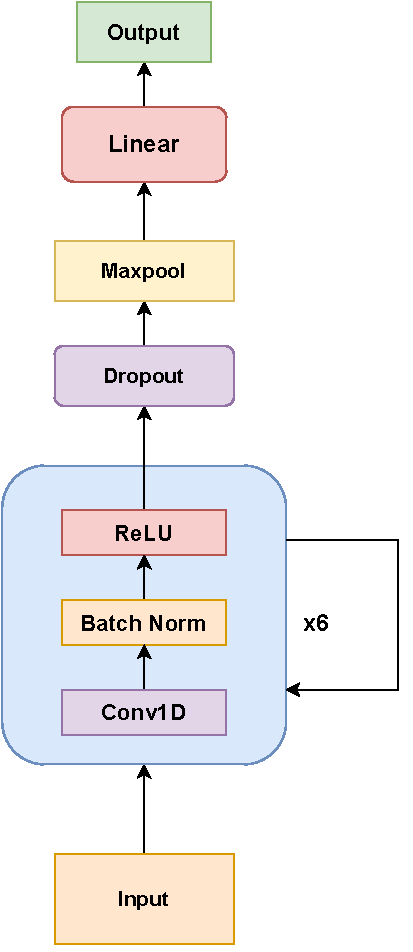
\includegraphics{images/fig_chapter2/nns/cnn_mt.pdf}
    \caption{Convolutional Neural Network Used}
    \label{fig:cnn_used}
\end{figure}

\subsection{ResNet}
Convolution neural network having \textbf{Residual Skip Connections} with six \textbf{1D-Convolutional} Layers in sequence with \textbf{Batch Normalisation} and  \textbf{ReLU} activation is used to extract features from the input data. Then the output of these convolution layers is regularized using \textbf{dropout} and down-sampled using \textbf{Max-pooling}. Finally, pose is regressed using a series of two fully connected \textbf{Linear} layers. 

\subsubsection{Model Output Analysis}
Figure xx shows the model output vs ground truth plot for a 27 seconds video in all 6 DoF (3 Linear and 3 Angular Displacement). The model can regress stabilization trajectory based on input IMU readings with good precision but there are zones where the prediction is off and thus causes jitter in stabilization. The error in all DoF can be seen in figure xx.

\begin{figure}
    \centering
    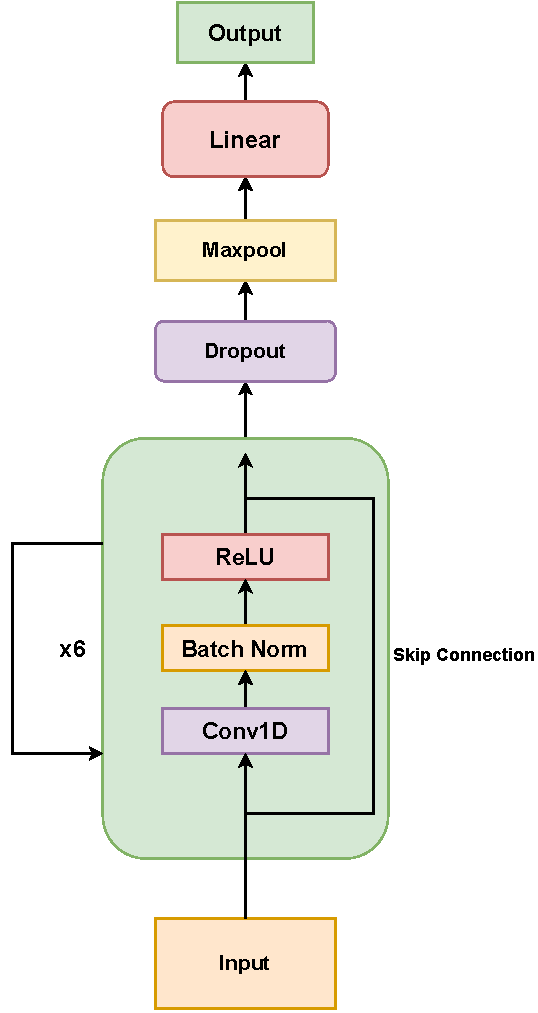
\includegraphics{images/fig_chapter2/nns/resnet_mt.pdf}
    \caption{CNN with Residual Skip Connections}
    \label{fig:resnet_used}
\end{figure}

\subsection{CNN-Transformer}
The network is structured in a way that the input goes through four \textbf{1D-Convolutional Layers} in sequence with \textbf{GELU} activation (non-linear). The output from these convolutional layers is fed to the \textit{Transformer Encoder}. Transformer Encoder has six layers with each layer having \textbf{Multi Headed Attention}, \textbf{Dropout}, \textbf{GELU} and \textbf{Layer Norm}. The output from the encoder layer goes into the output layers consisting of \textbf{Layer Normalization}, \textbf{Linear} layer, \textbf{GELU} non-linearity, \textbf{Dropout} and finally a \textbf{Fully Connected} layer to regress the output pose.

\subsubsection{Model Output Analysis}
Figure xx shows the model output vs ground truth plot for a 27 seconds video in all 6 DoF (3 Linear and 3 Angular Displacement). The model can regress stabilization trajectory based on input IMU readings with very precision and the error is in a very low range of the order of micrometers ($ \mu m $) and micro radians ($ \mu \theta $).

\begin{figure}
    \centering
    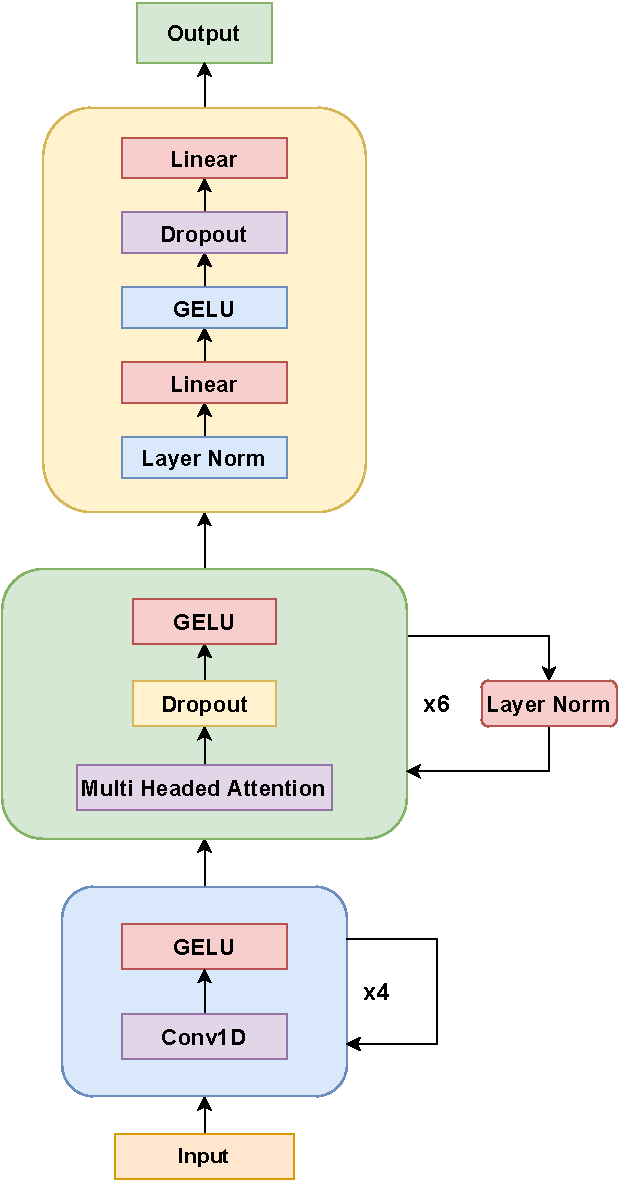
\includegraphics{images/fig_chapter2/nns/transformer_mt.pdf}
    \caption{CNN-Transformer Network Used}
    \label{fig:cnn_transformer_used}
\end{figure}


\section{Video Stabilization}
We will see the Stabilized Videos and discuss about how they look visually to different people.

\begin{sidewaysfigure}
    \centering
    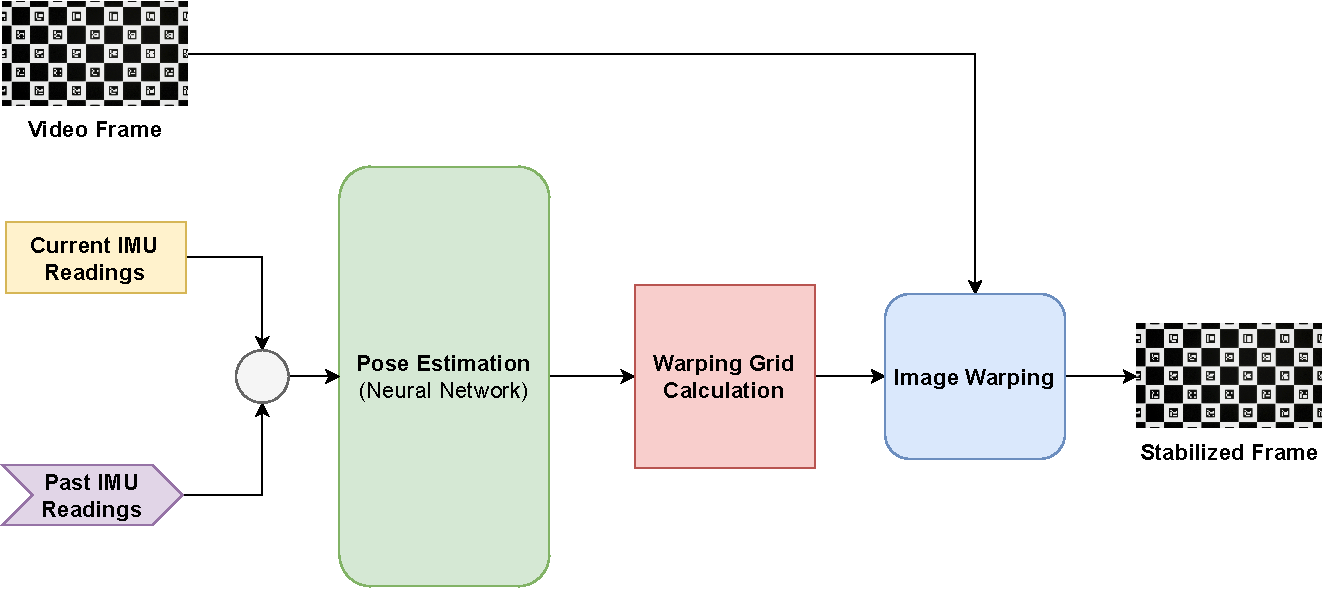
\includegraphics[scale=0.9]{images/fig_chapter4/dis_pipleline.pdf}
    \caption{DIS pipeline using IMU Sensor}
    \label{fig:dis_pipeline}
\end{sidewaysfigure}

\subsection{Smoothening of Stabilization Trajectory}

\begin{sidewaysfigure}
    \centering
    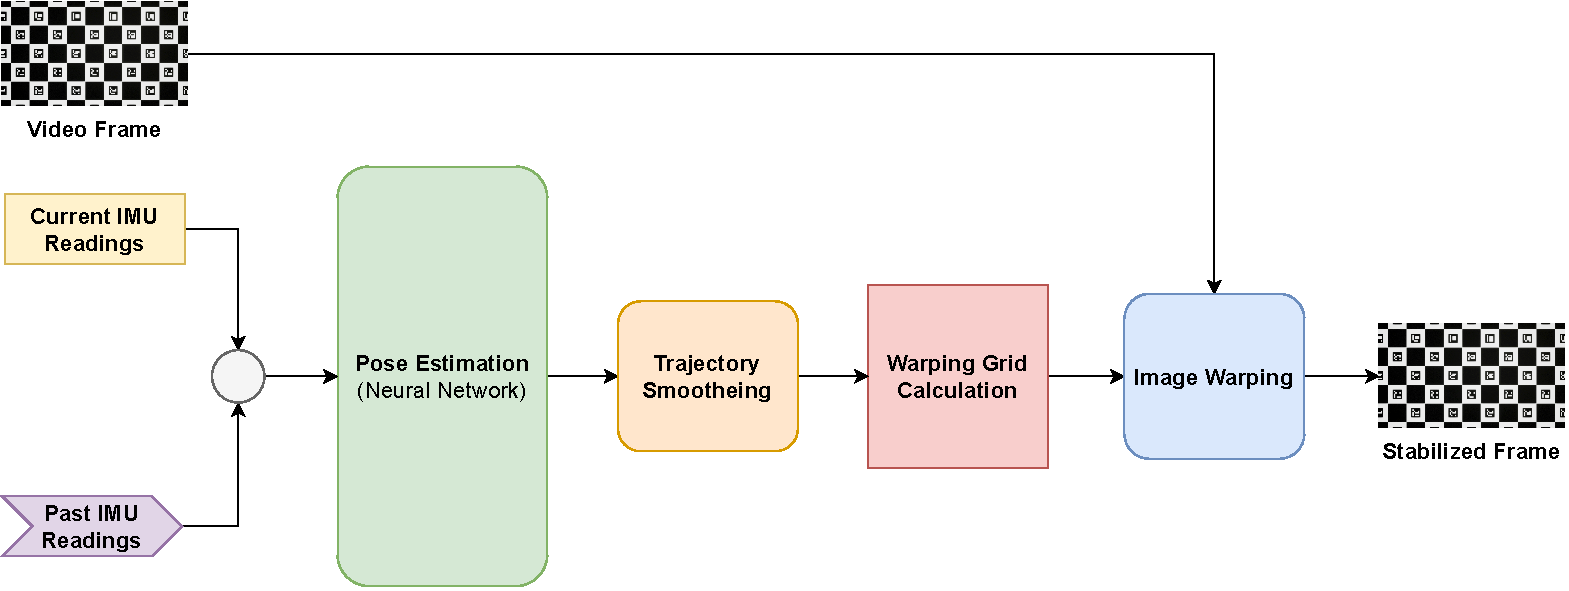
\includegraphics[scale=0.78]{images/fig_chapter4/dis_smooth_pipeline.pdf}
    \caption{DIS Pipeline with Trajectory Smoothening}
    \label{fig:dis_smooth_pipeline}
\end{sidewaysfigure}

\section{Model Deployment}
Figure \ref{fig:dis_smooth_pipeline} shows the digital image stabilization pipeline and our goal is to minimise the time taken at each step. The video (images) are coming at 60 FPS from the camera have 4K resolution (3840x2160 pixels). We ideally have 1/60 seconds (16.67 ms) to complete all the steps of the DIS pipeline. In this pipeline, Model Inference and Stabilization grid calculation take most of the given time. Stabilization grid calculation is a series of matrix multiplications and has been already optimized. Thus, low inference latency is highly desirable.

\subsection{Making Models Fast}
There are many techniques to reduce the inference latency of neural network models. Using these methods may reduce the performance of a neural network but are essential for deployment as models in their original form may not be usable at all. Some of the popular methods are discussed below.

\subsubsection{Altering Model Weights}
This is a very common approach used to to tackle high latency of deep learning models especially in case of edge hardware deployment. We can \textbf{quantize} the model by by converting the weights from floating point (32-bits) to integers (8 bits). This decreases the memory requirements significantly while also improving CPU and hardware accelerator latency \citep{FastModels}. 

Another recent approach is to convert the model to \textbf{half-precision} (16-bit floating point). It acts as a middle ground between FP32 and INT8 and the performance trade-off is reduced while decreasing the model size. Another very important thing to note is that not all layers have high latency and thus selective weight altering for layers like convolution layers can also be done making the performance trade-off even smaller.

\subsubsection{Making Models Lean}
The field of deep-learning is growing at a very high rate and we have a large selection of various neural network architectures some even with more than 100 Billion trainable parameters. But while developing deep-learning models, our goal should be to use models with the lowest number of parameters and complex layers while keeping the performance acceptable. The smaller the model is the better its inference latency. 
\subsection{Model Inference Latency on various Hardware}
Various trained models (CNN, ResNet and Transformer) are checked for inference latency and the results are summarised in table x. Models were also quantized or converted to ONNX for deployment. The models were inferred 1000 times and the result in the table is an average.

% Sim Vibration characteristics
 \begin{table}[ht]
\centering
\begin{tabular}{ l | L | L | L }
    
    Architecture  & 
    Format & 
    No. of Parameters &
    Inference Latency (ms) \\
    \hline
    
    CNN & 
    PyTorch Checkpoint (.ckpt)  & 
    00  &
    00  \\
    
    
    CNN & 
    ONNX (.onnx)  & 
    00  &
    00  \\
    
    ResNet & 
    PyTorch Checkpoint (.ckpt)  & 
    00  &
    00  \\
    
    
    ResNet & 
    ONNX (.onnx)  & 
    00  &
    00  \\
    
    CNN-Transformer & 
    PyTorch Checkpoint (.ckpt)  & 
    00  &
    00  \\
    
    
    CNN-Transformer & 
    ONNX (.onnx)  & 
    00  &
    00  \\
    
    
      
    
    \hline
   
\end{tabular}
    \caption{Inference Latency of Models}
    \label{tab:model_inference}
\end{table} %%%%



% 5. Chapter: ''Realisation and Evaluation''
\chapter{Results and Discussions} \label{chapter_five}

\begin{itemize}
\item Which method worked the best?
\item What was the effect of data structuring? 
\item Is the stabilisation good enough?
\item Was data enough Domain Randomised?
\end{itemize}

% The chapters Introduction and Conclusions have NO sections
% For the other chapters:
% Each sectioning (chapter, section, subsection, ...) should have NONE
% or AT LEAST TWO sub parts!
%\section{First Section}
%\subsection{First Subsection}
%\subsubsection{First Subsubsection}
%\paragraph{First Paragraph.} Some content for the first paragraph. 
%\subparagraph{First Subparagraph.} Some content for the first subparagraph. 
% Please note the dot after the paragraph and subparagraph heading. This is not accidently.

%Use bibtex for references to literature. 
%The most references will be in the second chapter.

% Make the references section
\bibliography{references} % According to the name of your bib file

% Start the appendix
\appendix
%%%%%%%%%%%%%%%%%%%%%%%%%%%%%%%%%%%%%%%%%%%
%  Place appendix content here            %
%  or use \input{appendix/appendixname}   %
%%%%%%%%%%%%%%%%%%%%%%%%%%%%%%%%%%%%%%%%%%%
\chapter{First Appendix Chapter}
\section{First Appendix Section}
\subsection{First Appendix Subsection}
\subsubsection{First Appendix Subsubsection}

\cleardoublepage

%----------------------------------------------------------------------------------------
%	DECLARATION PAGE
%---------------------------------------------------------------------------------------

% TODO uncomment the next three lines if your thesis is wirtten in german 
% \chapter*{Eidesstattliche Erklärung}
% \markboth{Eidesstattliche Erklärung}{Eidesstattliche Erklärung}
% \addcontentsline{toc}{chapter}{Eidesstattliche Erklärung}

% TODO comment the next three lines if your thesis is written in german 
\chapter*{Declaration of Authorship}
\markboth{Declaration of Authorship}{Declaration of Authorship}
\addcontentsline{toc}{chapter}{Declaration of Authorship}
% TODO Change the declaration according as needed. 

I hereby declare that I have written the above {\thesistype} thesis report independently and that I have not used any sources or aids other than those indicated. 

\bigskip

\begin{tabular}{@{}l@{}}
  Jena, Germany \rule[-0.8em]{7em}{0.5pt}\\[2ex]
  ~
\end{tabular}
\hspace{\fill}%
\begin{tabular}{@{}c@{}}
  \rule[-0.8em]{19em}{0.5pt}\\[2ex]
  {Ibad Rather}
\end{tabular}\hspace{\fill}

% Finish content and document
\end{document}
